\documentclass[draft]{agujournal2018}
\usepackage{apacite}
\usepackage{url} %this package should fix any errors with URLs in refs.
\usepackage{lineno}

\linenumbers
%%%%%%%
% As of 2018 we recommend use of the TrackChanges package to mark revisions.
% The trackchanges package adds five new LaTeX commands:
%
%  \note[editor]{The note}
%  \annote[editor]{Text to annotate}{The note}
%  \add[editor]{Text to add}
%  \remove[editor]{Text to remove}
%  \change[editor]{Text to remove}{Text to add}
%
% complete documentation is here: http://trackchanges.sourceforge.net/
%%%%%%%

%\draftfalse

%% Enter journal name below.

\journalname{JGR: Solid Earth}


%\documentclass[extra,mreferee]{gji}

%\documentclass[extra]{gji}

%\includeonly{sensPSV}

\usepackage{amsmath,amssymb,amsfonts,graphicx,subfigure,bm,yfonts,cleveref}
\usepackage{rotating}
%\usepackage[outdir=./]{epstopdf}

\usepackage{multirow}

%%%%%%%%%                              DEFINITIONS START

\def\cpar{$C_{ij},\rho$ parameterization~}
\def\hpar{h-parameterization~}

\newcommand{\todo}[1]{{\textbf {\color{red} #1}}}
\newcommand{\done}[1]{{\bf {\color{green} #1}}}


\def\rmrk#1{{\textbf{[[#1]]}}}
\def\rmrkok#1{}
%\def\eqref#1{\ref{#1}}
\def\eqrf#1{equation~\eqref{eq:#1}}
%\def\eqref#1{equation~\ref{eq:#1}}
\def\eq{equation~}
\def\figref#1{Fig.~\ref{fig:#1}}

\def\fref#1{\ref{#1}}


%\def\rmrk#1{{[\textcolor[rgb]{0,0,0.8}{#1}]}} % [blue]
%\def\rmrkm#1{{\textbf{[[\textcolor[rgb]{{1.00,0.00,0.00}}{#1}]]}}}
% _____________________________________________________________________________
\def\mainauthor{Vladimir Kazei}
\def\coauthorb{Ekkehart Tessmer}
\def\coauthorc{}%Zedong Wu
\def\coauthora{Tariq Alkhalifah}
% - my definitions==============================================================================================

\def\DP{Diffraction-based radiation 
patterns }
\def\dP{diffraction-based radiation 
patterns }

\def\nt{N}
\newcommand{\Mod}[1]{\ (\mathrm{mod}\ #1)}
\def\dv{\mathbf{d}}
\def\Amat{\mathbb{A}}
\def\Rmat{\mathbb{R}}
\def\Umat{\mathbb{U}}
\def\Smat{\mathbb{S}}
\def\Vmat{\mathbb{V}}
\def\SF{R}
\def\xv{\mathbf{x}}
\def\mv{\mathbf{m}}
%\def\tmul{\otimes}
\def\tmul{}
\def\cv{\mathbf{c}}

\def\sp{\varsigma}
\def\spv{\bm{\sp}}
\def\gp{\xi}
\def\gpv{\bm{\gp}}

\newcommand{\nmz}[1]{\mathbf{\bar{\text{$#1$}}}}
%\def\nmz#1{\mathbf{\bar #1}}

\def\Uv{\mathbf{U}}
\def\kv{\mathbf{k}}
\def\sv{\mathbf{s}}
\def\svn{\mathbf{\bar{\sv}}}
\def\Sv{\mathbf{S}}
\def\Gv{\mathbf{G}}
\def\Cv{\mathbf{C}}
\def\ev{\mathbf{e}}
\def\gv{\mathbf{g}}
\def\gvn{\mathbf{\bar{\gv}}}
\def\Av{\mathbf{A}}
\def\Bv{\mathbf{B}}
\def\uv{\mathbf{u}}
\def\rv{\mathbf{r}}
\def\dxv{\Delta \mathbf{x}}
\def\Kv{\mathbf{K}}
\def \cost{ \cos \frac{\theta}{2}}
%\newcommand{\sdot}{\mathbf{\bullet}}

\newcommand{\sdot}{{WI-WS, \delta \mv}}

\newcommand{\inty}{\int\limits_{-\infty}^{+\infty}}
\newcommand{\intyt}{\inty\inty\inty}
\newcommand{\intyV}{\int\limits_{V}}

\def\Rp{\mathcal{R}}
\def\Dp{\mathcal{D}}
\def\Tp{\mathcal{T}}
%\def\Cp{\mathcal{C}}
\def\Sp{\mathcal{S}}

% - Tariq's definitions begin here ==============================================================================
\def\beq{\begin{eqnarray}}
\def\eeq{\end{eqnarray}}

\def\mmbx#1{{\mathbf{#1}}}

\def\phi{\varphi}

\def\Vv{\mmbx{V}}
\def\gammav{\pmb{\gamma}}
\def\epsv{\pmb{\eps}}
\def\deltav{\pmb{\delta}}
\def\etav{\pmb{\eta}}

\def\v{V}
\def\rhov{\pmb{\rho}}
\def\r{\mmbx{r}}
\def\k{\mmbx{k}}

\def\d{\text{d}}
\def\c{\mmbx{c}}
\def\e{\mmbx{e}}
\def\m{\mmbx{m}}
\def\x{\mmbx{x}}
\def\xs{\x_s}
\def\xr{\x_r}
\def\L{\mmbx{L}}
\def\p{\mmbx{p}}
\def\q{\mmbx{q}}

\def\La{{\cal L}}
\def\tf{\tilde{f}}
\def\tA{\tilde{A}}
\def\ttau{\tilde{\tau}}
\def\y{\mmbx{y}}
\def\z{\mmbx{z}}

\def\tm{\tilde{m}}
\def\tr{\tilde{r}}
\def\tw{\tilde{w}}
\def\tv{\tilde{v}}
\def\tp{\tilde{p}}
\def\tq{\tilde{q}}

\def\a{\mmbx{a}}
\def\H{\mmbx{H}}
\def\g{\mmbx{g}}
\def\W{\mmbx{W}}

\def\eps{\varepsilon}

\def\La{{\cal L}}

\def\tlambda{\tilde{\lambda}}
\def\tw{\tilde{w}}

\def\rvn{r_{v_n}}
\def\rvh{r_{v_h}}
\def\rrho{r_\rho}
\def\rdel{r_\delta}
\def\reta{r_\eta}
\def\reps{r_\eps}


\def\Re{{{\cal{R}}_e}}

\newcommand{\pd}[2]{\frac{\partial #1}{\partial #2}}

%==============================================end of Tariq's notation=========================================


%%%%%%%%%								DEFINITIONS END
\newcommand{\mylabel}[1]{\label{#1}}
\newcommand{\myrf}[1]{\ref{#1}}

\newcommand{\plot}[3]{
	\begin{figure}
		\center
		\includegraphics[#2]{Fig/#1}
		\caption{#3}
		\label{fig:#1}
	\end{figure}
}

\newcommand{\twplot}[3]{
	\begin{figure}
		\centering
		\subfigure[]{\includegraphics[width=0.95\columnwidth]{Fig/#1}
			\label{fig:#1}}
		\hspace*{-0.01\columnwidth}
		\subfigure[]{\includegraphics[width=0.45\columnwidth]{Fig/#2}
			\label{fig:#2}}
		\caption{#3}
		%\label{fig:#1}
	\end{figure}
}

\newcommand{\tplot}[4]{
	\begin{figure}
		\centering
		\subfigure[]{\includegraphics[width=0.32\columnwidth]{Fig/#1}
			\label{fig:#1}}
		\vspace*{-0.01\columnwidth}
		\subfigure[]{\includegraphics[width=0.32\columnwidth]{Fig/#2}
			\label{fig:#2}}
		\vspace*{-0.01\columnwidth}
		\subfigure[]{\includegraphics[width=0.32\columnwidth]{Fig/#3}
			\label{fig:#3}}
		\caption{#4}
		\label{fig:#1_#3}\label{fig:#1_Full}
	\end{figure}
}

\newcommand{\fplot}[5]{
	\begin{figure}
		\centering
		\subfigure[]{\includegraphics[width=0.48\columnwidth]{Fig/#1}
			\label{fig:#1}}
		\hspace*{-0.01\columnwidth}
		\subfigure[]{\includegraphics[width=0.48\columnwidth]{Fig/#2}
			\label{fig:#2}}
		\hspace*{-0.01\columnwidth}
		\subfigure[]{\includegraphics[width=0.48\columnwidth]{Fig/#3}
			\label{fig:#3}}
		\hspace*{-0.01\columnwidth}
		\subfigure[]{\includegraphics[width=0.48\columnwidth]{Fig/#4}
			\label{fig:#4}}
		\caption{#5}
		\label{fig:#1:#4}\label{fig:#1_Full}
	\end{figure}
}

\newcommand{\fiPlot}[6]{
	\begin{figure}
		\centering
		\subfigure[]{\includegraphics[width=0.31\columnwidth]{Fig/#1}
			\label{fig:#1}}
		\hspace*{-0.01\columnwidth}
		\subfigure[]{\includegraphics[width=0.31\columnwidth]{Fig/#2}
			\label{fig:#2}}
		\hspace*{-0.01\columnwidth}
		\subfigure[]{\includegraphics[width=0.31\columnwidth]{Fig/#3}
			\label{fig:#3}}
		\hspace*{-0.01\columnwidth}
		\subfigure[]{\includegraphics[width=0.33\columnwidth]{Fig/#4}
			\label{fig:#4}}
		\subfigure[]{\includegraphics[width=0.33\columnwidth]{Fig/#5}
			\label{fig:#5}}
		\caption{#6}
		\label{fig:#1:#5}\label{fig:#1_Full}
	\end{figure}
}

\newcommand{\dplot}[3]{
	\begin{figure}
		\centering
		\subfigure[]{\includegraphics[width=0.49\columnwidth]{Fig/#1}
			\label{fig:#1}}
		\hspace*{-0.01\columnwidth}
		\subfigure[]{\includegraphics[width=0.49\columnwidth]{Fig/#2}
			\label{fig:#2}}
		\vspace*{-0.01\columnwidth}
		\caption{#3}
		\label{fig:#1:#2}\label{fig:#1_Full}
	\end{figure}
}

\newcommand{\ddplot}[3]{
	\begin{figure}
		\centering
		\subfigure[]{\includegraphics[width=0.7\columnwidth]{Fig/#1}
			\label{fig:#1}}
		\hspace*{-0.01\columnwidth}
		\subfigure[]{\includegraphics[width=0.99\columnwidth]{Fig/#2}
			\label{fig:#2}}
		\vspace*{-0.01\columnwidth}
		\caption{#3}
		\label{fig:#1_#2}\label{fig:#1_Full}
	\end{figure}
}

\def\ewidth{0.4}


\newcommand{\eplot}[9]{
	\begin{figure}
		\centering
		\subfigure[]{\includegraphics[width=\ewidth\columnwidth]{Fig/#1}
			\label{fig:#1}}
		\hspace*{-0.01\columnwidth}
		\subfigure[]{\includegraphics[width=\ewidth\columnwidth]{Fig/#2}
			\label{fig:#2}}
		\hspace*{-0.01\columnwidth}
		\subfigure[]{\includegraphics[width=\ewidth\columnwidth]{Fig/#3}
			\label{fig:#3}}
		\hspace*{-0.01\columnwidth}
		\subfigure[]{\includegraphics[width=\ewidth\columnwidth]{Fig/#4}
			\label{fig:#4}}
		\hspace*{-0.01\columnwidth}
		\subfigure[]{\includegraphics[width=\ewidth\columnwidth]{Fig/#5}
			\label{fig:#5}}
		\hspace*{-0.01\columnwidth}
		\subfigure[]{\includegraphics[width=\ewidth\columnwidth]{Fig/#6}
			\label{fig:#6}}
		\hspace*{-0.01\columnwidth}
		\subfigure[]{\includegraphics[width=\ewidth\columnwidth]{Fig/#7}
			\label{fig:#7}}
		\hspace*{-0.01\columnwidth}
		\subfigure[]{\includegraphics[width=\ewidth\columnwidth]{Fig/#8}
			\label{fig:#8}}
		\caption{#9}
		%\label{fig:#1}
	\end{figure}
}




\begin{document}

\title{Scattering Radiation Pattern Atlas: What anisotropic elastic properties can body waves resolve?}

%{Atlas of anisotropic elastic waveform inversion spectral resolution}

\authors{\mainauthor\affil{1}~\&~\coauthora\affil{1}}

\affiliation{1}{King Abdullah University of Science and Technology (KAUST), Thuwal, Saudi-Arabia}

\correspondingauthor{Vladimir Kazei}{vladimir.kazei@kaust.edu.sa}

%% Keypoints, final entry on title page.

%  List up to three key points (at least one is required)
%  Key Points summarize the main points and conclusions of the article
%  Each must be 100 characters or less with no special characters or punctuation

% Example:
% \begin{keypoints}
% \item	List up to three key points (at least one is required)
% \item	Key Points summarize the main points and conclusions of the article
% \item	Each must be 100 characters or less with no special characters or punctuation
% \end{keypoints}

\begin{keypoints}
	\item We share the resolution limits for each anisotropic parameter in waveform inversion
	\item For orthorhombic and VTI media we map the null-space of the inversion
	\item Converted waves are necessary to move the inversion beyond monoclinic anisotropy type
\end{keypoints}


\begin{abstract}
%Multiparameter full-waveform inversion is one of the most modern and widespread fields of study in modern geophysics. 
%
%Elastic anisotropic assumption is one of the most relevant physics for wavefield modeling and inversion.
%
Full-waveform inversion (FWI) optimizes the subsurface properties of geophysical earth models in such a way that the modeled data, based on these subsurface properties, match the observed data. The anisotropic properties, whether monoclinic, orthorhombic, triclinic, or vertical transversally isotropic (VTI), of the subsurface, be it a fractured reservoir or the core-mantle boundary, are necessary to describe the observed wave phenomena. In principle, there are no limitations on the complexity of the anisotropy that can be inverted using FWI. However, the question remains - what kind of anisotropic descriptions of the elastic properties of the earth can or cannot be inverted reliably from full seismic waveforms? We reveal the resolution that can be achieved through reconstructions of each elastic parameter by building vertical resolution patterns from the scattering radiation patterns. A visual analysis of these patterns indicates "tradeoffs", i.e., perturbations of parameters that have the same reflection-based scattering patterns as other perturbations. Each tradeoff leads to an apparent ambiguity in the inversion results, which must be addressed by additional assumptions, constraints, or regularizations. For orthorhombic media, we find the exact tradeoffs that exist between parameters. Our parameterization isolates the VTI parameters and, therefore, we also obtain the null-space of every scattering mode for VTI media. We also discover that only monoclinic parameters are recoverable from the first order scattering of monotypic waves. We summarize the tradeoffs found in tables for easy reference. This paper is intended to be useful for researchers setting up anisotropic FWI problems and quality control of such inversions.
\end{abstract}

%least how many model constraints do we need to make the inversion meaningful?
%The answer is important in both exploration and global seismology as 
%it guides us to what we can invert for and at what resolution.
%
%Let us consider a simple experiment: a small anisotropic scatterer illuminated from all sides by certain wave mode(s). 

%We don't know the scatterer properties 
%distribution, just assume that it's small enough to fit into the Born 
%scattering assumption. We try to answer a simple question:
%%
%%what do we primarily propose as a solution?
%%
%We employ scattering radiation patterns in order to attain such information 
%When the scatterer is a point with respect to the dominant wavelength, the scattered energy is described by
%diffraction-based radiation patterns. Otherwise, if the 
%shape of the scatterer is not restricted, reflection-based radiation patterns 
%can be remapped into the spectral domain and used for the parameter 
%reconstruction. Thus, we provide a table describing 
%fundamentally irresolvable tradeoffs between parameters in weakly anisotropic 
%media. The resolution and accuracy depends on the noise level. 
%So in a singular value decomposition analysis linear parameter combinations with values that fall below the noise level cannot be properly inverted for.
%
%We show that if there is no tilt in the background vertical variations of it are not recoverable.

%As a result, such tradeoffs can be mitigated through appropriate 
%constraints during an anisotropic inversion process and present an estimate of 
%the number of distributed parameters recoverable in single mode inversions for 
%orthorhombic anisotropic media. We develop multiparameter inversion resolution analysis 
%and in particular design better parameterizations and regularizations for such 
%inversions.


%Reflection-based radiation patterns are remapped into the normalized 
%wavenumber domain to access resolvability of anisotropic elastic parameters at 
%different scales. Particularly we focus on scattering by orthorhombic 
%parameters, which represent upscaled carbonate reservoir geology most accurate 
%and dominate over lower anisotropies in the Earth's crust. We utilize singular 
%value analysis of the spectral sensitivities to reveal numerical null-spaces 
%for data of only certain wave modes and some of their practical combinations. 
%Three component measurements of explosive source scattered waves theoretically 
%allow to decouple all ten orthorhombic parameters. Density is included, unlike 
%in some previous studies on elastic scattering. 

\section{Introduction}
% what is the problem?
% The problem is that anisotropic parameters are coupled
%\subsection{Anisotropy in the earth}
A realistic representation of propagating wavefields is key to creating accurate subsurface 
models in global and exploration seismology.
%
Elastic anisotropy, which can be classified and decomposed based upon the symmetries present in the anisotropic media \citep{browaeys2004,bona2007}, strongly influences the propagation of wavefields throughout the earth's interior.
%
In global seismology, inversions of the anisotropy of the inner core 
\citep{tromp1993support,creager1999large} and some regions of the earth's 
mantle \citep[e.g.,][]{long2010mantle,bozdag2016} have been used to construct more realistic 
global models for a better understanding of the physics of the earth. However, it is difficult to predict the optimal constraints, regularizations, and parameterizations to apply when designing elastic anisotropic inversions.

Tradeoffs are another major challenge encountered when inverting the anisotropic elastic 
properties of the earth's subsurface. Tradeoffs, also called couplings, between anisotropic parameters occur when different combinations of parameter perturbations lead to almost identical scattering patterns, i.e., the different perturbations produce the same elastic wave recordings. The problem of parameter tradeoffs is not new and has been  
extensively studied in isotropic media 
\citep{wu1985,tarantola1986,virieux2009,kohn2012,anikiev2014m,vegard2017}, vertical transversally isotropic (VTI) media \citep{eaton1994,gholami20131,alkhalifah2014,plessix2016}, and 
orthorhombic media \citep{hoop1999,shaw2004,juwon2016,kazei2017}. %\cite{} 
\cite{kohn2015} performed a synthetic feasibility investigation on FWI for all triclinic elastic parameters, excluding density from the inversion.  
In this paper, we address the tradeoffs that inevitably arise in general elastic anisotropic inversions by explicitly defining those combinations that lead to similar recordings.
%
%\subsection{Common types of anisotropy}

We consider the four most common cases of seismic anisotropy: VTI, orthorhombic (orthotropic), monoclinic, and triclinic anisotropy.
VTI anisotropy is naturally induced in the subsurface by gravity-related vertical stress \citep{thomsen1986} and thin layering.
%
Transversally isotropic media have one axis of rotational symmetry, which is often vertical. Therefore, the body waves propagate with the same velocity in any horizontal direction, but have different velocities depending on the deviation of the propagation direction from vertical (angle $\theta$ in \figref{orthoReservoir}).
%Transversally isotropic anisotropy with arbitrary orientations, e.g., horizontal transversally isotropic(HTI) and tilted transversally isotropic(TTI), is the common limitation of most modern studies.
Orthorhombic anisotropy characterizes most fractured carbonate reservoirs \citep{schoenberg1997,tsvankin1997} and, therefore, plays a dominant role in exploration seismology. Orthorhombic anisotropy is also found in olivine crystals \citep{durham1977}, which comprise a significant part of the earth's mantle and deeper crust \citep[e.g.][]{tommasi2009}.
% 
An orthorhombic medium can be viewed as a combination of two transversally isotropic media, one with a vertical axis of symmetry (layering) and another with a horizontal axis of symmetry (e.g., fractures). Wave propagation in such a medium depends on the azimuth (angle $\phi$ in \figref{orthoReservoir}).
% 
Even the kinematics of wave propagation in orthorhombic media are rather complicated and the subject of much current research \citep{stovas2015,stovas2017,ivanov2016,xu2018}. Monoclinic anisotropy is sometimes found in more complex geological formations or multiple sets of fractures \citep{grechka2000}. A triclinic anisotropic medium, the most common in the earth, has no planes of symmetry. Any elastic solid can be described by twenty-one elastic constants and density -- triclinic anisotropic media require all twenty-two of these parameters for a complete description. Unfortunately, independent inversion for all twenty-two parameters is still a big challenge \citep{kohn2015} due to various tradeoffs. We try to understand which parameters are principally recoverable from different types of scattering and at which resolution.

The paper is organized as follows. 
In Section 2, we provide the history and general properties of scattering functions and the diffraction, reflection, and transmission of scattering radiation patterns. In Section 3, we introduce spectral sensitivities in order to directly access the vertical resolution lengths in inversion. In Section 4, we provide an atlas of these sensitivities for all possible parameter perturbations and all scattering modes. We also reveal the null-spaces for each scattering mode and verify those null-spaces analytically using a numerical singular value decomposition (SVD) analysis. In Section 5, we summarize the tradeoffs in two tables and show how three-component data can be utilized to determine all the orthorhombic parameters based on null-space intersections.

\twplot{orthoReservoir}{CijMap}{Orthorhombic reservoir. a) Anisotropic fractured reservoir (small black box with vertical planes) in isotropic background. Arrows indicate incident and scattered waves, $\theta$ denotes the incidence angle and $\phi$ the azimuth of the reflection plane w.r.t. the symmetry plane of the reservoir.  b) Elements of stiffness matrix in Voigt notation \citep[e.g.][p. 8--15]{babuska1991}. Only red and blue cells are non-zero for monoclinic media with horizontal ($x_1$ - $x_2$) plane of symmetry. In orthorhombic media only nine (in red) parameters are non-zero (if the symmetry planes are $x_1-x_2, x_1-x_3, x_2-x_3$).}









%is the ultimate goal of elastic 

%If there are no planes of symmetry for the elastic solid triclinic anisotropy is the most general kind of anisotropy found in the earth. %For this reason, it is the ultimate destination of inversion methods not reached by FWI yet \citep{kohn2015}. 
%Triclinic
%\subsection{Null-space, coupling and tradeoff in multiparameter inversion}
%


 



%what do we add?
%\subsection{What is missing?}
%Some modern seismic exploration surveys include full azimuth coverage, extended bandwidth and multi-component measurements, have the potential to improve quality and quantity of the resolvable information and allow for lower symmetry anisotropy types to be considered for inversion. Similar situations occur in regional and global seismology when dense networks such as US Array \citep{gao2006upper,zhu2017} and additional sensors are placed into the ocean \citep{simons2009potential,sukhovich2015seismic}.
%%


%Relying on spectral analysis, we try to answer a simple question for general 
%anisotropic media, with more details for isotropic, VTI and orthorhombic cases: 
%What kind of anisotropy would we be able to invert just from particular 
%scattered wave modes or at least how many constraints do we need to make 
%the inversion meaningful?
%
% e first provide a fundamental analysis based on the case in which we have perfect illumination.


%

%\subsection{Outline}





%


%scattering radiation patterns in order to answer these questions and 
%in the end of the paper provide a table describing fundamentally irresolvable 
%tradeoffs between parameters. These tradeoffs need to be eliminated by 
%constraints during an anisotropic inversion process.

%The most well-known reductions of the function, characterized by four angles, 
%are the diffraction scattering pattern, the reflection scattering pattern, and 
%the transmission scattering pattern.  
%Non-scattering linear combinations of radiation patterns represent couplings 
%of 
%parameters that are fundamentally irresolvable.




%




% 
%for spectral domain
%\cite{wu:11} mapped scattering into the spectral domain \cite{mora1989} mapped 
%the 
%\cite{kazei2013gp,kazei2013spectral} found the parts of the patterns 
%activated by head and diving waves.

	
\section{Scattering radiation patterns of elastic parameters}

We give a brief history of patterns and then describe them mathematically.
We start the mathematical description with the scattering function introduced by \cite{eaton1994}, which describes the scattering of arbitrary plane waves on a point scatterer, and we discuss its reduction to diffraction-based 
\citep{wu1985,tarantola1986} and reflection-based 
\citep{gholami20131,alkhalifah2014} scattering radiation patterns.

\subsection{Brief history of scattering radiation patterns}

%\rmrk{VT: Section 2 should start here}
We consider a multiparameter inverse problem of perfect illumination, where a small anisotropic scatterer is illuminated from all directions. We do not know the scatterer, but we have recorded a certain scattered wave mode, e.g., $P-P$ scattered waves.
% 
The function that depends on incident and scattered wavefields directions and describes the ratio between scattered and incident wavefield amplitudes is the scattering radiation pattern \citep{wu1985,alkhalifah2014}. 
%,podgornova,kamath2016,masmoudi2016,juwon2016,kazei2017,kazei2018}. %  
Using these radiation patterns, which are known from the recorded wave mode, we try to infer the scattering parameter of the scatterer.
%



%
% what has been done?
%
%Evaluation of the scattering radiation patterns through the Born approximation is 
%natural, because the Born approximation represents the leading term of the scattering series and is at the heart of modern seismic 
%imaging techniques such as waveform tomography, FWI and LSRTM.
%
%\subsubsection{In isotropic media}


Different types of radiation patterns indicate different types of elastic 
parameter perturbations and, therefore, can help to distinguish among the parameters from seismic data. \cite{wu1985} described radiation patterns for isotropic elastic 
parameters in the standard ($\lambda,\mu,\rho$) parameterization. 
%
\cite{tarantola1986} considered scattering in several parameterizations of 
isotropic elastic media. He came to the conclusion that a parameterization featuring density and both $P$ and $S$ wave impedances was the 
most promising for reflection seismic 
data. 
%
%\subsubsection{In anisotropic media}
\cite{eaton1994} introduced a scattering function that 
described the scattering of arbitrary plane waves on an arbitrary scatterer in background media with arbitrary anisotropy. 
\cite{hoop1999} focused on the resolvable 
parameters in orthorhombic media and were probably the first to implicitly use 
reflection-based radiation patterns 
\citep{gholami20131,alkhalifah2014,kamath2016,plessix2016}. \cite{juwon2016} 
analyzed 
scattering for several parameterizations of orthorhombic media and proposed a 
hierarchical parameterization, which we use throughout this paper, to reduce the tradeoffs between parameters.

% spectral domain
\subsection{Scattering angle - resolution length relation}

While radiation patterns characterize scattering for point perturbations, they 
can be generalized to arbitrary perturbations that fit into the Born 
approximation. If the scattering experiment is handled in the model wavenumber domain \citep{devaney1984}, then
we can access additional features of the scattering such as resolution (\figref{ksg}).
%
For acoustic monochromatic plane waves, there is a simple relation between 
the wavenumbers in the model and the scattering angles \citep{ewald1969,devaney1984}. 
\cite{wu:11} compared wavenumbers that are covered by scattered waves in vertical seismic profiling (VSP) 
and surface observations. \cite{mora1989} analyzed the contributions of reflections to the illuminated wavenumber spectrum in background media. \cite{kazei2013gp} 
provided a quantitative wavenumber illumination analysis of the spectrum covered by head waves and diving waves. \cite{podgornova,podgornova2018} analyzed 
the resolvability of elastic parameter spectra in elastic VTI media. 
\cite{kazei2018} presented spectral coverage and resolution for orthorhombic 
parameters. 
%
\begin{figure}
	\centering
	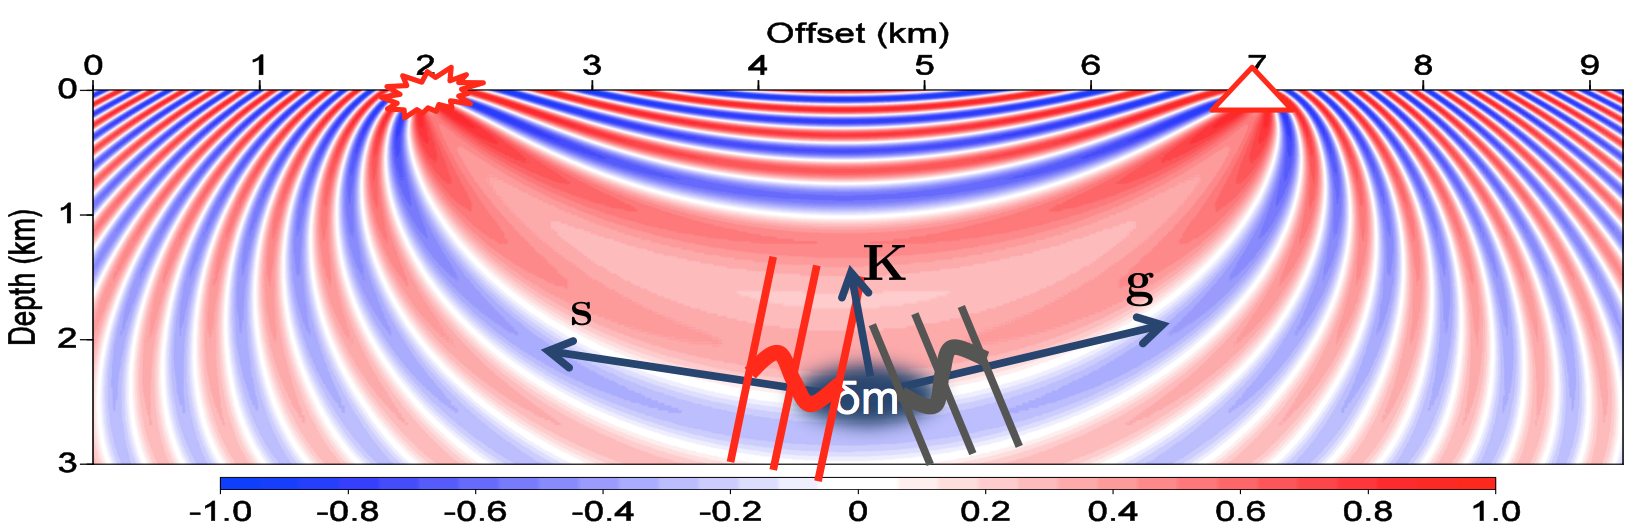
\includegraphics[width=0.9\linewidth]{Fig/Ksg}
	\caption{Sensitivity kernel for the frequency domain in a linearly increasing velocity background \citep{alkhalifah2014scattering,kazei2016}. $\Kv = \omega(\sv+\gv)$. With a decrease in the scattering angle (the angle between slowness vectors towards the source $\sv$ and receiver $\gv$), the resolution length $L \propto |\Kv|^{-1}$ also decreases.}
	\label{fig:ksg}
\end{figure}

In our previous work \citep{kazei2018}, we performed an analysis of the 
radiation patterns describing the scattering of $P$ waves on orthorhombic 
parameters in an isotropic, homogeneous-medium background. Here, we present a similar 
analysis for different types of scattering. Namely, we consider $S$ waves and 
$P-S$ conversions. In order to access the scattering caused by isotropic and VTI 
parameter perturbations, we use a hierarchical parameterization based on that of 
\cite{juwon2016, kazei2018}.

\subsection{Scattering function}
A monochromatic plane wave is defined by its phase, polarization, and 
propagation directions. The phase accumulated while traveling through 
a background medium is dropped in our analysis so that we can focus on the local scattering 
features. Therefore, here the scattered wavefield $\delta 
\Uv$ depends only on the incident plane-wave slowness vector $\sv$, the scattered plane-wave slowness vector $\gv$, the respective 
polarizations $\spv$ and $\gpv$, the frequency $\omega$, and the 
perturbation of the parameters 
$\delta \mv  = (\delta \rho(\xv), \delta \cv(\xv))^T$:
\beq
\delta \Uv \cdot \gpv  \propto \SF_{\delta \mv} (\sv,\gv, \spv, \gpv).
\eeq
%
The coefficient $\SF$, well known for its arbitrary point scatterers, is called the scattering function \citep{eaton1994, shaw2004, 
calvet2006, kazei2018}, and is defined as 
%
\beq \label{eq:sfun}
\SF_{\delta \mv} (\sv,\gv, \spv, \gpv) \equiv \sp_k \gp_k \delta \rho  + 
s_i \sp_j \delta c_{ijkl} g_k \gp_l 
\\
= \spv \cdot \gpv \delta \rho + \sv \tmul \spv : \delta \cv : \gv \tmul \gpv.
\eeq
While $\SF$ is \emph{independent} of the background medium, which can have up to triclinic-anisotropy complexity, eight 
different angles determine the directions of polarization and propagation for its incident and scattered wavefield (there are four directions, featuring two angles each). 
Thus, there are many possibilities for polarization and propagation relations in a general anisotropic background as well as for velocities of incident and scattered waves; here, we consider scattering in an isotropic background.
 
%Instead of expressions including angles we try to stick with vector notation to keep it more compact.

\subsection{Classic diffraction-based scattering radiation pattern -- $\Dp$} 
A general anisotropic medium allows for nine types of plane-wave scattering, 
each characterized by four independent angles that represent directions of 
propagation.
For a given incident and scattered wave type in an isotropic background (e.g., $P-P,~ P-SV,~SV-SV,~SV-SH$, 
etc.), the scattered wavefield becomes a function of the two vectors $\sv$ and 
$\gv$. This function is the diffraction-based radiation pattern:
\beq
\Dp_{WI-WS, \delta \mv}(\sv,\gv) \equiv \frac{ \SF (\sv, \gv, \spv(\sv, WI), \gpv (\gv, WS), \delta \mv)}{||\delta \mv||}.
\eeq
Here, $WI$ denotes the type of incident waves, and $WS$ denotes the type of scattered 
waves ($P-P, P-S_i, S_i-P$, or $S_i-S_j$) for a given parameter perturbation 
$\delta \mv$. 



\DP characterize the scattering of certain 
types of plane waves on a point-like perturbation of the parameters. For example, in the case of $P-P$ ($WI=WS=P$) scattering in an isotropic background 
\begin{align}
\spv(\sv, \sdot) &= \sv,~ 
\gpv (\gv, \sdot)  = \gv 
\end{align}

on a $\lambda$ 
perturbation,
%\beq
\begin{align}
	\delta c_{ijkl} = \delta_{ij} \delta_{kl} \delta \lambda, ~
	WI-WS &= P-P, ~
	\delta \rho = 0,~ \delta m = \delta \lambda \\
	\Dp_\sdot (\sv,\gv) &= \Dp_{P-P,\delta\lambda} (\sv,\gv) = \frac{1}{\v_p^2}.
\end{align}
For vertically propagating incident $P$ waves, the scattering radiation 
patterns become functions of two real arguments, which are $\gv$ vector components, 
and can be presented as a 2D plot \citep{eaton1994}.


\DP were examined by \cite{wu1985,tarantola1986,beylkin1990} for isotropic 
parameters, 
%\rmrk{VT: need commas not semi colons for this list}, 
and by \cite{calvet2006} for VTI parameters in the classic \cite{thomsen1986}
parameterization. For isotropic parameters in an isotropic background, the full
scattering information can be recovered by a single  diffraction-based  radiation  pattern, as the only 
important parameter in that case is the difference between the incident and 
scattered directions \citep{wu1985,tarantola1986}. This is not the case in anisotropic media \citep[e.g.,][]{eaton1994,calvet2006,juwon2016}. We illustrate the dependence of the invoked source at the scatter location on the incidence using the example of the $C_{55}$ and $C_{12}$ elements shown in \figref{patterns/C_55/PP_diffZ_Full}. The dependence of the diffraction patterns on the four angles describing the source and receiver directions complicates further analysis. To complete our analysis, we must reduce the diffraction-based patterns to reflection and transmission scattering radiation patterns. 

\fplot{patterns/C_55/PP_diffZ}{patterns/C_55/PP_diffXYZ}{patterns/C_13/PP_diffZ}{patterns/C_13/PP_diffXYZ}{Diffraction-based radiation pattern for $P-P$ scattering and perturbation in $C_{55}$ and $C_{13}$ for vertical and oblique ($\sv = \frac{1}{\sqrt{3}\v_p}(1, 1, 1)^T$) incidence. $C_{55}$ does not scatter vertically incident waves -- (a), but scatters for out of symmetry plane incidence -- (b). $C_{13}$ works like an X-axis expansion source for vertical incidence and like expansion source in XZ plane for oblique incidence -- (d).}



\subsection{Reflection-based radiation patterns -- $\Rp$}
Classic \dP describe diffractions from point scatterers. However, seismic 
surveys are commonly dominated by reflections (\figref{orthoReservoir}). Therefore, linearized reflection coefficients 
\citep[e.g.,][]{ruger1997} and, more recently, reflection-based radiation patterns 
\citep{shaw2004,gholami20131,alkhalifah2014} were developed. A given wave-mode relation 
between the reflection-based radiation patterns and the reflection coefficients can be reduced to a scattering angle-dependent coefficient, which is independent of the scatterer 
type \citep{shaw2004}.
%
In 3D scattering experiments, scattering functions depend on four scalar 
parameters, which are defined by unit vectors $\sv$ and $\gv$. For a plane reflector, 
the scattered wave direction is determined by the incident direction through Snell's law, and vice 
versa. Similarly, the dip and azimuth of the reflector determine how 
vector $\sv$ is tied to vector $\gv$ through Snell's law, reducing 
the number of real variables that determine scattering from four to two:
%
\beq \label{eq:reflPat}
\Rp_{WI-WS, \delta \mv}(\gv) \equiv \Dp_{WI-WS, \delta \mv}(\sv(\gv),\gv). 
\eeq
%
The amplitude of the reflections from perturbations of isotropic parameters does 
not depend on the reflector orientation; therefore, the reflection-based 
radiation patterns are the same for all reflector orientations. For anisotropic 
reflectors and backgrounds, the reflection-based radiation patterns depend on 
the dip and azimuth angles. In most seismic cases, the medium is dominated by 
horizontal layering. For this reason, we follow the example of \cite{gholami20131} and \cite{alkhalifah2014}, and focus on scattering from horizontal reflectors. We illustrate typical reflection-based radiation patterns for $C_{ij}$ parameters in \figref{patterns/C_55/PP_reflZ_Full}.

 

\fplot{patterns/C_55/PP_reflZ}{patterns/C_13/PP_reflZ}{patterns/C_16/PP_reflZ}{patterns/C_36/PP_reflZ}{Reflection-based radiation patterns for $P-P$ scattering and $C_{55}$ -- (a), $C_{13}$ -- (b), $C_{16}$ -- (c), $C_{36}$ --(d). Just by looking at the radiation patterns we can state that $C_{13}$ and $C_{55}$ can not be determined together at high precision as they scatter in a very similar if not identical way.}





\section{Wavenumber illumination theory}
In the previous section, we discussed the scattering of plane waves on point 
scatterers. But reflection-based radiation patterns can be 
remapped into the frequency-wavenumber domain in order to accommodate the scattering effects of any arbitrary perturbations that fit into the Born approximation.
%
\cite{ewald1969} spheres have been used to recognize the relation between illuminated wavenumbers in a perturbation and the directions of its incident and scattered waves in monochromatic plane-wave experiments. 
For example, \cite{devaney1984} used this 
method to quantify the resolution of geophysical diffraction tomography images in the
wavenumber domain. This technique was later applied to acoustic FWI scenarios 
for surface seismic acquisition \citep{mora1989} and vertical seismic profiling 
\citep{wu:11}. \cite{kazei2013gp} introduced the amplitude of the spectral 
sensitivity of the data to the perturbations of various background media, and applied it to models with diving waves and multiples \citep{kazei2015seg,kazei2013spectral}. An elastic isotropic-background case 
with VTI perturbations was considered by \cite{podgornova}. Here, we show the 
applicability of this technique to arbitrary anisotropic perturbations of isotropic media. 
%
% 
%The possibility of recovering a set of parameters is defined by the sensitivity 
%of the scattered wavefield to these parameters. Under the plane-wave 
%assumption, the resolution is straightforward for the wavenumber domain 
%representation of perturbation.
%For single wave mode we could compare reflection-based radiation patterns to 
%understand the coupling effects.


In this section, we provide a derivation of the 
scattering function and 
generalize it to spectral sensitivities 
\citep{kazei2013gp,podgornova,kazei2017}.
%
By incorporating the spectral sensitivities, we can consider a broad class of anomalies 
so small that we can neglect the second-order scattering. 
%
 

%For instance, mapping into wavenumber domain allows to consider 
%information 
%available for inversion from $P-P$ and $P-SV$ waves together.
% 
\subsection{Far-field plane-wave scattering}
Radiation patterns simply represent different types of scattered wavefields for a point scatterer 
when the far-field or plane-wave approximation is applied to \eqrf{hudson} below. While the derivation is well-known, we return to it in order to generalize the radiation patterns to arbitrary scatterers that 
satisfy \eqrf{hudson}. First, we utilize the approximation from the receiver 
side of \eqrf{hudson}, since it includes Green's tensors and not incident 
wavefields. Then, we treat the source wavefields in the same manner.

\subsubsection{The Born approximation}
We consider an incident wavefield $\Uv^0$ on a perturbation of the density ($\delta\rho(\xv)$) and stiffness tensor ($\delta c_{kjpq}(\xv)$) parameters.
The frequency-domain Born approximation for the scattered wavefield $\delta \Uv$ in an anisotropic elastic medium is \citep[e.g.,][]{hudson1981,beylkin1990,shaw2004}
\beq \label{eq:hudson}
\delta U_i (\xv_s,\xv_\gv,\omega) = \intyV  (\delta \rho(\xv) U^0_k \omega^2 - 
\delta c_{kjpq}(\xv) \pd{U^0_p}{x_q}  \pd{}{x_j})G_{ik}(\xv_g, \xv) \d \xv,
\eeq
where $\omega$ is the angular frequency, $\xv_s$ and $\xv_g$ are the coordinates of the source and receiver, respectively, and $G_{ik}(\xv_g, \xv)$ is the Green's tensor for the background medium. Integration is performed over the volume of the perturbation $\delta \mv = (\delta \rho, \delta c_{ijpq})$, where $\mv$ is the vector of unperturbed parameters. 
We can vectorize the equation~\eqref{eq:hudson},
\beq \label{eq:hudsonVec}
\delta \Uv (\xv_s,\xv_\gv,\omega) = \intyV  (\omega^2 \delta \rho(\xv) \Uv^0 (\xv) \cdot\Gv (\xv) - 
\nabla \Gv (\xv) : \delta \cv(\xv) : (\nabla \Uv^0 (\xv))   \d \xv,
\eeq
which already gives us some insights into scattering. For example scattering on density perturbation is determined by the kernel 
\beq
\omega^2 \delta \rho(\xv) \Uv^0 (\xv) \cdot\Gv (\xv),
\eeq 
and hence depends only on the amplitudes and polarization of incident $\Uv^0$ and scattered $\Gv$ wavefields. For instance if we consider scattering of $SH$ waves in a vertical plane on density the amplitude of the scattered wavefield will be constant \figref{SHSH/SHSHCij}. At the same time scattering on perturbations of elastic constants $C_{ij}$ driven by the kernel
\beq
\nabla \Gv (\xv) : \delta \cv(\xv) : (\nabla \Uv^0 (\xv))
\eeq
can as well depend on the propagation directions
of incident and scattered waves, which are extracted by the gradient $\nabla$ operator.
 
\subsubsection{Wavefields scattered by perturbation}
The Green's tensor $G_{ik}$ in the Born approximation~\eqref{eq:hudsonVec} physically 
takes care of the propagation of a scattered wavefield from the perturbation to the 
receiver.
The far-field approximation for the Green's tensor \citep[e.g.,][]{snieder2002} in a homogeneous, isotropic background 
%is
%\begin{align} \label{eq:farField}
%	\Gv(\xv,\xv_g) &= \alpha\bigg(  e^{i\frac{\omega}{\v_p}||\xv - \xv_g||} \gv\gv
%	\\
%	&+\frac{1}{\varkappa^2} e^{i\frac{\omega}{\v_s}||\xv - \xv_g||} (\gv_{\theta}\gv_{\theta} + \gv_{\phi}\gv_{\phi})\bigg), 
%	\varkappa = \frac{\v_s}{\v_p}, \alpha = \frac{1}{4\pi\rho \v_p^2||\xv - \xv_g||},
%\end{align}
%where $\gv,~\gv_{\theta},$ and $~\gv_{\phi}$ are the polarization vectors of the $P$, $SV$, and $SH$ waves, respectively. Thus, the far-field part of the Green's tensor (26) 
consists of $P,~ SV,$ and $SH$ waves:
\beq \label{eq:3G}
\Gv(\xv_g, \xv) = \alpha (\Gv_P(\xv_g, \xv) + \Gv_{SV}(\xv_g, \xv) + \Gv_{SH}(\xv_g, \xv)). 
\eeq
While $SV$ and $SH$ waves in isotropic media most often come together, they are usually recorded separately and therefore can be analyzed separately too. 
The coefficient 
\beq
\alpha = \frac{1}{4\pi\rho \v_p^2||\xv - \xv_g||}.
\eeq
is dropped in our resolution analysis, since it is related to geometrical spreading and can be effectively compensated using pseudo-hessian techniques. Different components of the Green's function are approximated locally by plane waves. For the first component $\Gv_P$, the approximation leads to
\beq \label{eq:GvP}
\Gv_P = e^{i\frac{\omega}{\v_p}||\xv_g- \xv ||} \gvn\gvn \simeq 
e^{i\frac{\omega}{\v_p}\gv\cdot(\xv - \xv_g)}\gvn\gvn, ~ 
\gvn = \frac{\gv}{|\gv|} = \frac{\xv-\xv_g}{|\xv-\xv_g|},
\eeq
which is the $P$ wave approximated by a plane wave at the location $\xv$. ($\gv\gv)_{ik} = g_i g_k$ denotes standard outer product of vector $\gv$ with itself. 
%For the second and third 
%components, $\Gv_{SV}$ and $\Gv_{SH}$, similar expressions can be provided 
%\citep{snieder2002}.
The second component, $\Gv_{SV}$, represents a shear wave polarized in the vertical plane 
that contains $\xv$ and $\xv_g$:
\beq \label{eq:GvSV}
\Gv_{SV} = \frac{1}{\varkappa^2} e^{i\frac{\omega}{\v_s}||\xv - \xv_g||}\gv_{\theta}\gv_{\theta} \simeq 
\frac{1}{\varkappa^2} e^{i\frac{\omega}{\v_s}\gv\cdot(\xv - \xv_g)}\gv_{\theta}\gv_{\theta},~
\gv_\theta = \left( \frac{\gv \times \ev_z}{|\gv \times \ev_z|}\times \gvn \right). 
\eeq
Finally, the third component of the Green's tensor, $\Gv_{SH}$, is an $SH$ wave polarized along $\gv_\phi$:
\beq \label{eq:GvSH}
\Gv_{SH} = \frac{1}{\varkappa^2} e^{i\frac{\omega}{\v_s}||\xv - \xv_g||}\gv_{\phi}\gv_{\phi} \simeq 
\frac{1}{\varkappa^2} e^{i\frac{\omega}{\v_s}\gv\cdot(\xv - \xv_g)}\gv_{\phi}\gv_{\phi},
\gv_\phi = \left( \frac{\gv \times \ev_z}{|\gv \times \ev_z|}\right),
\eeq
which is the horizontal component of a shear wave.
%\subsubsection{Incident wavefield}

For the incident wavefield we consider point forces in three directions $\svn, \sv_\phi, \sv_\theta$, leading to three respective wavetypes:
\beq \label{eq:P_sou}
\Uv_{0P} = \Gv_P(\xv_s,\xv) \cdot \svn,
\eeq
\beq
\Uv_{0SV} = \Gv_{SV}(\xv_s,\xv) \cdot \sv_\theta,
\eeq
\beq
\Uv_{0SH} = \Gv_{SH}(\xv_s,\xv) \cdot \sv_\phi.
\eeq
%\cite{walter2007} analyzed the empirical relations between the amplitudes of $P$ 
%and $S$ waves emitted by explosive sources and double-couple earthquake sources, and came to the conclusion that $P$ waves dominate the explosions, while $S$ waves dominate the earthquakes.

%For simplicity, we consider incident plane waves with unit amplitudes:
%\beq
%\Uv_0 = \Av_0 \exp(i \kv_s \cdot \xv),
%\eeq
%where $\Av_0$ and $\kv_s$ represent the polarization and wavenumber vectors, respectively, of an incident wave.
%For $P$ waves,
%\beq \label{eq:P_sou}
%\Av_0 = \svn,~ \kv_s=\frac{\omega}{\v_p}\svn, \svn = \frac{\xv_s-\xv}{|\xv-\xv_s|}.
%\eeq
%For $SV$ waves,
%\beq
%\Av_0 = \sv_\theta,~ \kv_s=\frac{\omega}{\v_s}\svn,~
%\sv_\theta =  \left( \frac{\sv \times \ev_z}{|\sv \times \ev_z|}\times \svn
%\right).
%\eeq
%For $SH$ waves,
%\beq
%\Av_0 = \sv_\phi,~ \kv_s=\frac{\omega}{\v_s}\svn,~
%\sv_\phi = \left( \frac{\sv \times \ev_z}{|\sv \times \ev_z|}\right).
%\eeq


%
%\input{theory/born}
%
\subsection{Model wavenumbers and scattering modes}
We start with scattered $P$ waves as they are the easiest to handle and by far the most popular in FWI applications. By substituting equations \eqref{eq:P_sou} and \eqref{eq:GvP} into equation \eqref{eq:hudson}, and projecting the scattered wavefield $\Uv$ onto the direction of $\gv$ (from the perturbation to the receiver), we obtain the approximate amplitude of the scattered $P-P$ waves \citep{kazei2018} as
\beq \label{eq:UPPInt}\label{eq:UPPInt1}
\delta U_{PP} = \delta \Uv_P \cdot \svn  \propto 
%\frac{\delta \mathbf{U} \cdot \gv}{\alpha_{PP}} \simeq
\intyV   e^{i\Kv \cdot \xv} (\svn\cdot\gvn \delta \nmz{\rho} (\xv) + \svn\svn : \delta 
\nmz{\cv}(\xv) :\gvn\gvn) \d \xv, 
\eeq
where
%\beq 
%\alpha_{PP} = \frac{\omega^2}{v^2_p} \alpha_s \alpha_g e^{i\frac{\omega}{\v_p}(-\xv_s\sv-\xv_g\gv)}
%\eeq
%and
\beq \label{eq:K}
\Kv = \omega(\sv+\gv).
\eeq

Analogously, for the amplitude of the scattered $P-SV$ waves, we use equations \eqref{eq:P_sou} and \eqref{eq:GvSV}, and project \eqref{eq:hudson} onto vector $\gv_{\theta}$ to obtain
\beq \label{eq:UPSVInt}
\delta U_{PSV} = \delta \Uv_P \cdot \sv_\theta 
\propto   
%\frac{\delta \mathbf{U} \cdot \gv_\theta}{\alpha_{PS}} \simeq\frac{1}{\varkappa^3}
\intyV  e^{i\Kv_{PS}\cdot\xv} (\svn\cdot\gv_{\theta} \delta \nmz{\rho} + \frac{1}{\varkappa} \svn\svn : \delta \nmz{\cv} :\gvn\gv_{\theta}) \d \xv. 
\eeq
%where
%\beq
%\alpha_{PS} = \frac{\alpha_{PP}}{\varkappa^3} e^{i\omega\gv_\theta \cdot (\frac{\xv_g}{\v_p}-\frac{\xv_g}{\v_s})}, \Kv_{PS}=\frac{\omega}{\v_p}\sv+\frac{\omega}{\v_s}\gv.
%\eeq

Replacing the polarization vector $\gv_\theta$ in (39) with $\gv_\phi$ is sufficient to obtain similar expressions for the $P-SH$ scattering scenario. For $S$ waves, we obtain similar expressions by using equations \eqref{eq:P_sou}, \eqref{eq:GvSH}, and \eqref{eq:hudson}:
\beq \label{eq:USHSHInt}
\delta U_{SHSH} = \delta \Uv_{SH} \cdot {\sv_\phi} 
\propto 
%\equiv  \frac{\delta \mathbf{U} \cdot \gv_\phi}{\alpha_{SS}} \simeq \frac{1}{\varkappa^3}
\intyV  e^{i\Kv_{SS}\cdot\xv} (\sv_\phi \cdot \gv_\phi \delta \rho + \frac{1}{\varkappa^2} \nmz{\sv}\sv_\phi : \delta \nmz{\cv} :\nmz{\gv}\gv_{\phi}) \d \xv. 
\eeq
%where
%\beq
%\alpha_{SS} = \frac{\alpha_{PP}}{\varkappa^6} e^{i\omega\gv \cdot (\frac{\xv_g}{\v_s}-\frac{\xv_g}{\v_s})}, 
%\Kv_{SS}=\frac{\omega}{\v_s}(\sv+\gv).
%\eeq

For different types of scattering, our further resolution analysis is based on equations 
(\ref{eq:UPPInt1}-\ref{eq:USHSHInt}) and their analogs, which describe the monochromatic scattering of $P$ waves.

 

Different scattering modes contribute to different wavenumbers at 
the same reflection angle and frequency of the image. Therefore, in order to investigate all the
information available, we need to remap the reflection-based radiation patterns into 
the spatial wavenumber domain. Equation \eqref{eq:K} governs the mapping procedure and \figref{K_PP_Full} illustrates how it defines the resolution of the different types of body wave scattering.

\tplot{K_PP}{K_PS}{K_SS}{For the same incident angle 
	and same temporal frequency different modes provide illumination to different 
	vertical wavenumbers. (a) $P-P$ waves illuminate the lowest wavenumbers (good for FWI), 
	(c) $S-S$ waves -- the highest wavenumbers (good for migration), and (b) $P-S$ waves -- the intermediate wavenumbers.}

We note that the right-hand sides of equations \eqref{eq:UPPInt1}, \eqref{eq:UPSVInt}, and \eqref{eq:USHSHInt} are essentially Fourier transforms of the perturbation. Thus, we can generalize these equations as 
\beq \label{eq:KvMain}
\delta U_{WI-WS}(\sv,\gv,\omega) \propto \spv\cdot\gpv \delta \hat{\rho}(\Kv_{WI-WS}(\sv,\gv,\omega)) + \sv\spv : \delta \hat{\cv}(\Kv_{WI-WS}(\sv,\gv,\omega)) :\gv\gpv.
\eeq
Equation~\eqref{eq:KvMain} shows that for a given scattering mode, the wavenumber resolved by inversion depends only on the frequency, source and receiver directions. On the other hand, we can infer all possible directions towards the source and receiver for a given wavenumber. Analyzing scattering for these directions leads directly to irresolvable tradeoffs in inversion at a particular length.

%In single mode scattering considerations, the coefficient $\varkappa^{-3}$ can 
%be dropped \citep{podgornova}. 

%but in order to consider the information 
%available from several wave types together we need to take it into account:
%\beq \label{eq:alphaPPPS}
%|\alpha_{PS}| = \varkappa^{-3}|\alpha_{PP}|
%\eeq
%\beq
%\label{eq:incident}
%\kv_g = \frac{\omega}{v_{WS}}\gv,  \kv_s = \frac{\omega}{v_{WI}}\sv.
%\eeq


%



	


We note that the right-hand sides of equations \eqref{eq:UPPInt1}, \eqref{eq:UPSVInt}, and \eqref{eq:USHSHInt} are essentially Fourier transforms of the perturbation. Thus, we can generalize these equations as 
\beq \label{eq:KvMain}
\delta U_{WI-WS}(\sv,\gv,\omega) \propto \spv\cdot\gpv \delta \hat{\rho}(\Kv_{WI-WS}(\sv,\gv,\omega)) + \sv\spv : \delta \hat{\cv}(\Kv_{WI-WS}(\sv,\gv,\omega)) :\gv\gpv.
\eeq
Equation~\eqref{eq:KvMain} shows that for a given scattering mode, the wavenumber resolved by inversion depends only on the frequency, source and receiver directions. On the other hand, we can infer all possible directions towards the source and receiver for a given wavenumber. Analyzing scattering for these directions leads directly to irresolvable tradeoffs in inversion at a particular length.

Vertical variations are often dominant in subsurface structures in exploration seismology; therefore, we focus on the vertical wavenumbers $\Kv_{WI-WS}$ in the next section.

%In single mode scattering considerations, the coefficient $\varkappa^{-3}$ can 
%be dropped \citep{podgornova}. 

%but in order to consider the information 
%available from several wave types together we need to take it into account:
%\beq \label{eq:alphaPPPS}
%|\alpha_{PS}| = \varkappa^{-3}|\alpha_{PP}|
%\eeq
%\beq
%\label{eq:incident}
%\kv_g = \frac{\omega}{v_{WS}}\gv,  \kv_s = \frac{\omega}{v_{WI}}\sv.
%\eeq

\subsection{Vertical wavenumber sensitivity}

In this section, we construct sensitivities for vertical wavenumbers $\Kv = (0,0,K_z)^T$.
%
For a given frequency $\omega$ and a particular scattering mode, we can find the corresponding source and receiver directions and remap the radiation patterns into the normalized wavenumber-angle domain using 

\beq \label{eq:sensDef}
\Sp_{WI-WS,\delta \mv} (k_z, \varphi) \equiv \Dp_{\delta \mv, WI-WS} (\sv(k_z,\varphi,WI-WS), \gv(k_z,\varphi,WI-WS)),~
\eeq
where
\beq
k_z = \frac{K_z}{k_0},~
k_{0} = \frac{\omega}{\v_s}. 
\eeq
Equation (44) defines the spectral sensitivity for parameter 
$\delta \mv$. We normalize all the wavenumbers, dividing them by $\omega/V_s$. %acknowledging that the sensitivities scale linearly with 
%frequency in homogeneous backgrounds \citep{kazei2013gp}.
%We focus on the inversion for vertical wavenumbers $\kv_{PP}=(0,0,k_z)$, or horizontally layered structures, which are dominant in most geological scenarios, including those in the global scale, returning us to the remapped reflection-based radiation patterns in a more convenient representation for resolution analysis domain. 
These remapped patterns are functions of two variables ($k_z,\phi$) and, therefore, can be easily plotted and examined. 

\subsubsection{Snell's law in wavenumber domain}
For $S-S$ scattering, the vectors pointing towards the source and the receiver are easily found for a given $k_z\in [0,2]$:
\beq
s_1=-g_1=\frac{1}{V_s}\sqrt{1-\frac{k_z^2}{4}}\cos\phi,~ s_2=-g_2=\frac{1}{V_s}\sqrt{1-\frac{k_z^2}{4}}\sin\phi,~
s_3=g_3=\frac{1}{V_s} k_z/2.  
\eeq
For $P-P$ scattering on a horizontal reflector, the vectors pointing towards the source and the receiver are easily found for a given $k_z\in [0,2\varkappa]$:
\beq
s_1=-g_1=\frac{1}{V_p} \sqrt{1-\frac{k_z^2}{4 \varkappa^2}}\cos\phi,~ s_2=-g_2=\frac{1}{V_p} \sqrt{1-\frac{k_z^2}{4 \varkappa^2}}\sin\phi,~
s_3=g_3= \frac{1}{V_p} \frac{k_z}{2 \varkappa}.  
\eeq
The reflection-based radiation pattern for $C_{55}$ and $P-P$ scattering is represented in \figref{pattern_PP_reflZ}.

For $P-S$ scattering, Snell's law:
\beq
\sv +\gv = \Kv_z
\eeq
leads to the following expressions:
\beq
s_{xy} = \frac{1}{V_s} \sqrt{2\varkappa^2 k_z^2-\varkappa^4+2\varkappa^2-k_z^4+2k_z^2-1}/(2k_z),
\\
s_1=-g_1=s_{xy}\cos(\phi) ,~ s_2=-g_2=s_{xy}\sin(\phi), 
\\
s_3=\frac{1}{V_p}(\varkappa^2+k_z^2-1)/(2\varkappa k_z), g_3 = \frac{1}{V_s}(k_z^2-\varkappa^2+1)/(2k_z),
\eeq
where $\varkappa = \frac{\v_s}{\v_p}$ is the ratio of the shear and longitudinal velocities. 
We show all the possible reflection-based radiation patterns for other cases mapped from the $\phi,\theta$ domain into the wavenumber domain ($\phi,k_z$) as spectral sensitivities in order to directly access the resolution of inversion the normalized wavenumber domain.
%
This mapping allows us to compare wavenumbers and resolution covered by different wave types.

%
In the next section, we analyze the scattering of all the elastic 
constants and find the null-space of the inversion for each scattering mode.
 
\dplot{pattern_PP_reflZ}{PP_Full/PP_C_55}{(a) The reflection-based radiation pattern for $C_{55}$ and (b) its remapping into the spectral domain. The normalized wavenumber $||\Kv|| \propto \cos \theta_{max}$. In all the patterns, the amplitude sign is indicated by color: red corresponds to a positive reflection coefficient, i.e., no phase shift after scattering; blue shows a negative reflection or scattering coefficient.}


\section{Spectral sensitivities and numerical analysis of tradeoffs}
In the case of an isotropic background and a general anisotropic scatterer, there are six 
combinations of incident-scattered wave types and 22 elastic 
parameters to perturb. Thus, the total number of radiation patterns specified by 
$\sdot$ is 22*6=132, and this is the amount of data we need to analyze triclinic perturbations. In this section, we present the spectral sensitivities for all these 
parameters and discuss some features of the scattering modes case-by-case 
in the subsections. 

For the orthorhombic and VTI parameters, 
we find all the tradeoffs numerically with SVD and confirm them 
analytically.
Our SVD analysis of the radiation patterns answers the following 
questions:
%\rmrk{fix lists}
\begin{enumerate}
	\item What is the null-space of the linearized dynamic inversions?
	
	\item How many orthorhombic parameters can be resolved from a 
	given scattering mode?
\end{enumerate}
Of course, the answers to these questions depend on the method of acquisition and the signal-to-noise ratio of the data, assuming that coverage is perfect and there is no 
noise. Therefore, the tradeoffs we find are irresolvable.
% and other parameters coupling may exist in realistic illumination conditions.
%only and thus consider the following representative cases for the data components:
%\begin{enumerate}
%	\item $P-$waves only -- first arrivals.
%   \rmrk{next items in this list are removed from the story to simplify it}
%	\item $P$ and $P-SV$ waves.
%	\item $P-P,SV,SH$ -- full-waveform inversion.	
%\end{enumerate} 

\subsection{Sensitivity matrices $\Smat_{WI-WS}$ -- assembly}
In this subsection, we discuss the matrix form of the simplified inversion problem for the vertical wavenumber $\Kv$ from arbitrary scattering mode.   
%
For an arbitrary perturbation of parameters $\mv (\Kv)$, the scattered wavefield can be expressed in the wavenumber domain as
\vspace*{-0.02\columnwidth}
\beq \label{eq:Svec}
\delta U_{WI-WS} (k_z, \phi, \omega(k_z, K_z)) \propto \Sv_{WI-WS} (k_z, \varphi) \delta \mv (\Kv).
\eeq
Vector $\Sv_{WI-WS}(k_z,\phi)$ represents the set of reflection-based radiation patterns remapped into the normalized wavenumber domain. For example, element $S_1(k_z,\phi) \equiv \Sp_{WI-WS,\delta \nmz{\rho}}(k_z,\phi)$ is the radiation pattern of the density.

In matrix form, equation~\eqref{eq:Svec} can be written for all $(k_z,\phi)$ corresponding to a given $K_z$ together as follows:
\beq
\delta \Uv_{WI-WS}(K_z) \propto \Smat_{WI-WS} \delta \mv(K_z).
\eeq
Columns of the matrix $\Smat$ are, spectral sensitivities reshaped into vectors. Matrix $\Smat$ determines resolvability of parameters at a given spatial resolution. It's rank is equal to the maximum number of resolvable parameters. Matrix $\Smat$ can also be linked to the Hessian of standard full-waveform inversion \citep{kazei2018, podgornova2018}.

%
%The lack of high frequencies in the data activates the high wavenumber part of the spectral sensititivity and thus is similar to the case with low wavenumbers and the lack of offset too. The only difference between these two cases is what limits the maximum effective angle -- frequency or the aperture.

%\subsection{Combination of wavetypes}
%When several components of the wavefield are measured, several modes of scattering can be used together to retrieve particular wavenumbers. As a result, different frequencies and angles will be involved in the wavenumber inversion. In order to accommodate for that, we merge matrices $\Amat_{P-P}, \Amat_{P-SV}, \Amat_{P-SH}$ in normalized wavenumber $k_z$ domain, assuming same $k_z$ ranges for different wavetypes. The spectral sensitivities for these $k_z$ ranges are then concatenated into one matrix $\Amat$:
%\beq \label{eq:Amerge}
%\begin{pmatrix}
%	\delta \Uv_{P-P} \\
%	\delta \Uv_{P-SV} \\
%	\delta \Uv_{P-SH}
%\end{pmatrix} = \Amat \delta \mv, ~~~ 
%\Amat = 
%\begin{pmatrix}
%	\Amat_{P-P} \\
%	\Amat_{P-SV} \\
%	\Amat_{P-SH}
%\end{pmatrix}. 
%\eeq	
%Analogously the data for $P-P$ and $P-SV$ waves can be merged, if only vertical component at the ocean bottom is measured or is trustworthy for inversion. It is also possible to consider $P-P$ and $P-SH$, removing $P-SV$ components from the \eqrf{Amerge}, which is an interesting approach because $P-SH$ scattering happens only on parameters that are beyond VTI anisotropy.
%Then SVD analysis needs to be applied to $\Amat$ to determine the number and set of resolvable parameters.








\subsection{Hierarchical parameterization}

An FWI-suitable parameterization of orthorhombic media should describe isotropic media using only three non-zero parameters -- $V_p,V_s,$ and $\rho$. 

By adding three more parameters -- $\varepsilon_1, \eta_1,$ and $\gamma_1$ -- we can describe VTI media.

\todo{
Parameterization suggested by all and Alkhalifah features this separation of parameters into three groups. First group specifies parameters in isotropic medium. This parameters are standard and include PV velocity and S vein velocity and density. Second group brings in vertically transversely isotropic parameters. This group includes widespread in exploration and seismic parameterization by Alkhalifah and 20. Namely it includes Epsilon, gamma and eta. In this parameterization Epsilon describes the elliptic part of of anisotropy of P waves. Eta either corrects the anisotropy of P waves completely defeat their kinetics kinematics. The gamma parameter describes the anisotropy of SH waves. SV waves are thematically sensitive to the same parameters as P waves.
}







Finally, four additional parameters -- $\varepsilon_d, \eta_d, \gamma_d$, and $\delta_3$ -- allow us to go from VTI to orthorhombic anisotropy. This kind of parameterization is presented in \cite{juwon2016}.


Radiation patterns and the spectral sensitivities for any parameterization can be obtained through variable substitution to $C_{ij},\rho$ parameterization. 
\beq \label{eq:JacoCij}
\bm{\Rp}_{\mv, WT} = \bm{\Rp}_{\mv_0(\mv), WT} = \bm{\Rp}_{\pd{\mv_0}{\mv}\mv}
\eeq

The Jacobian $\pd{(\nmz{C}_{ij},\nmz{\rho})}{\mv}$ for the hierarchical parameterization has the following form:
\beq \label{eq:Jaco}
\delta \left(\begin{array}{c}
	 \nmz{\rho}  \\
	\nmz{C}_{11} \\
	\nmz{C}_{22} \\
	\nmz{C}_{33} \\
	\nmz{C}_{12} \\
	\nmz{C}_{13} \\
	\nmz{C}_{23} \\
	\nmz{C}_{44} \\
	\nmz{C}_{55} \\
	\nmz{C}_{66}
\end{array}\right)
= \left(
\begin {array}{cccccccccc} 
1 & 0 & 0 & 0 & 0 & 0 & 0 & 0 & 0 & 0 \\ 
1 & 2 & 0 & 0 & 0 & 0 & 0 & 0 & 0 & 0 \\ 
1 & 2 & 0 & 0 & 2 & 0 & 0 & 0 & 0 & 0 \\
1 & 2 & 0 & -2 & 0 & 0 & 0 & 0 & 0 & 0 \\ 
1-2\varkappa & 2 & -4\varkappa & 0 & 0 & 0 & 0 & 1 & -4\varkappa & 0 \\
1-2\varkappa & 2 & -4\varkappa & -1 & 0 & -1 & 0 & 0 & 0 & 0 \\
1-2\varkappa & 2 & -4\varkappa & -1 & 1 & -1 & -1 & 0 & 0 & -4\varkappa \\
\varkappa & 0 & 2\varkappa & 0 & 0 & 0 & 0 & 0 & 0 & 2\varkappa\\
\varkappa & 0 & 2\varkappa & 0 & 0 & 0 & 0 & 0 & 0 & 0 \\
\varkappa & 0 & 2\varkappa & 0 & 0 & 0 & 0 & 0 & 2\varkappa & 0
\end {array}
 \right)
\delta \left(\begin{array}{c}
	  \nmz{\rho}     \\
	 \nmz{V}_{p}     \\
	 \nmz{V}_{s}     \\
	 \eps_1    \\
	 \eps_d    \\
	 \eta_1    \\
	 \eta_d    \\
	\delta_3   \\
	\gamma_1   \\
	\gamma_d 
\end{array}\right)
\eeq
%
We also present the partial derivatives of the $C_{ij}$ parameters in a graph (\figref{PP_Full/parDerivCij}) to illustrate the perturbations in the elastic parameters that are introduced by perturbations from a single hierarchical parameter. To simplify formulas and focus on geometric properties of scattering we normalize units in the following way -- velocities are normalized by the background $\v_{p0}$, densities by $\rho_0$, elastic constants by $\rho_0 \v_p^2$. The normalized quantities are distinguished by the dash, e.g.
\beq
\nmz{\v}_p \equiv \frac{\v_p}{\v_{p0}}, 
\nmz{\v}_s \equiv \frac{\v_s}{\v_{p0}},
\nmz{C}_{55} \equiv \frac{C_{55}}{\rho\v^2_{p0}}. 
\eeq  

\plot{PP_Full/parDerivCij}{width=\columnwidth}{Partial derivatives of $C_{ij}$ parameters w.r.t. hierarchical parameterization parameters for $V_{0s}/V_{0p}=\varkappa=\frac{1}{\sqrt{3}}$.}


An advanced choice of parameterization will give some insights that are not straightforward from the $C_{ij}$ parameterization. For example, parameters contributing to $V_p$ provide zero sensitivity to $S$-wave scattering. Being a combination of nine $C_{ij}$ parameters, $V_p$ is hardly discoverable in the original parameterization. Thus, our knowledge is still limited by the choice of parameterization, as we cannot visually identify coupling among three or more parameters.


\subsection{$P-P$ scattering}
%
If registered, $P$ waves are the first waves that arrive at the receivers. Therefore, their travel times, or ``first breaks'', are the most common in seismic inversion setups.  The finite-frequency $P$-wave travel times are well represented by effective pseudo-acoustic 
modeling \citep{alkhalifah2000,wu2017}, though correct inversion of the amplitudes requires elastic-media representation even in isotropic media  
\citep{raknes2014,kurzmann2016}. In global seismology, the $P$ waves served as the main source of information about the core mantle and inner core--outer core boundaries for a long time \citep{bolt1970}. $P$ waves are still extensively exploited in inversions for the earth's inner core \citep{peng2008,yu2016,irving2015}, as well as for inversions of the mantle and crust. 
In our previous work, we analyzed the scattering of $P$ wave--scattered data with respect to the inversion opportunities \citep{kazei2018}; therefore, here we cover the decoupling of parameters in the case of perfect illumination only.

\ddplot{PP_Full/PPCij}{PP_Full/PPnPar0}{Spectral sensitivities to vertical 
wavenumbers for $P-P$ scattering on various $C_{ij}$ perturbations. Perturbations that scatter in a very similar manner are enclosed by frames of the same color. (a) Sensitivity to all $C_{ij}$ parameters and density perturbed independently. High wavenumbers for density resemble those for 
$C_{33}$, these are the only parameters scattering independently of the azimuth in the $C_{ij},\rho$ parameterization. Sensitivity to all monoclinic parameters is non-zero when we start from isotropic 
background. Yet, $C_{13}$ is very similar to $C_{55}$, $C_{12}$ to $C_{66}$, and 
$C_{23}$ to $C_{44}$.  Scattering by $C_{45}$ is similar to that by $C_{35}$. (b) In the 
hierarchical parameterization, $V_{s}$ is coupled to $\eta_1$, and $\eta_d$ is coupled to $\gamma_d$, finally, 
$\rho$ is very similar to $\epsilon_1$. The Poisson ratio is assumed to be 0.25 
($V_p/V_s = \sqrt{3}$).}
%

In \figref{PP_Full/PPCij} we see four non-orthorhombic elements that show non-zero 
sensitivity. These non-zero sensitivities can potentially be used to invert for a monoclinic medium or an orthorhombic medium that is rotated around the vertical axis. On the other hand, the sensitivity to tilts -- rotations around horizontal axis -- is zero; therefore, inversion for tilts from monotypic waves will not work for purely 
vertical wavenumbers.

Through SVD of the $\Amat$ matrix, each row represents a particular 
scattering experiment. Data at all angles in the radiation patterns are inverted 
together.
%
The number of parameters that are invertible is equal to the number of non-zero 
singular values in SVD.
%
The principal null-space is the span of singular vectors related to zero 
singular values. 
%
The graph of the singular values \figref{PP_Full/TotalSingVal} tells us how the condition number of the 
inverse problem decreases when we try to regularize inversion by reducing the 
number of parameters to be inverted.

We analyze the SVD of the full matrix $\Amat_{P-P}$ in the 
$C_{ij},\rho$ parameterization. \figref{PP_Full/TotalSingVal} shows that the 
matrix has only \emph{six} non-zero singular values and, thus, only \emph{six} 
independent parameters are invertible in this case. 
\figref{PP_Full/TotalSingVec1} shows the set of singular vectors in the 
$C_{ij},\rho$ parameterization. The numerical null-space is defined as the linear span of 
four singular vectors, corresponding to zero singular values (columns 7-10 in 
\figref{PP_Full/TotalSingVec1}). 
These vectors are
\beq
2\nmz{\Cv}_{12}-\nmz{\Cv}_{66}, \label{eq:C12C66}
\\
2\nmz{\Cv}_{13}+\nmz{\Cv}_{55},
\\
2\nmz{\Cv}_{23}+\nmz{\Cv}_{44},
\\
\nmz{\Cv}_{11}+\nmz{\Cv}_{12}+\nmz{\Cv}_{22}-\nmz{\Cv}_{33}+\nmz{\rhov}. 
\eeq
By substituting these combinations, which are found empirically, into the 
reflection-based radiation pattern expressions, \cite{kazei2018} showed that the inversion is not at all sensitive to them. 
For example
\begin{align}
\Rp_{2\nmz{\Cv}_{12}-\nmz{\Cv}_{66},P-P} \\ \nonumber
&= \Rp_{2\cv_{1122}-\cv_{1212}-\cv_{2121}-\cv_{1221}-\cv_{2112},P-P}(\sv,\gv) \\ \nonumber
&= 4 s_1s_1g_2g_2 - 4 s_1s_2g_1g_2 = 0.
\end{align}
%
We also found \citep{kazei2018} a particular combination of the stiffness matrix elements and density that does not produce reflections. The reflection-based radiation pattern of density can be transformed as follows:
\begin{align}
\Rp_{\pmb{\rho},P-P} =& \sv\cdot\gv \\ \nonumber
=& s_1g_1 + s_2g_2 + s_3g_3 \\ \nonumber
=& -s_1s_1-s_2s_2+s_3s_3 \\ \nonumber
=& -s_1s_1(s_1s_1+s_2s_2+s_3s_3) \\ \nonumber
&- s_2s_2(s_1s_1+s_2s_2+s_3s_3) \\ \nonumber
&+ s_3s_3(s_1s_1+s_2s_2+s_3s_3) \\ \nonumber
=& \Rp_{-\nmz{\Cv}_{11}-\frac{1}{2}(\nmz{\Cv}_{12}-\nmz{\Cv}_{13}),P-P} \\ \nonumber
&+ \Rp_{-\nmz{\Cv}_{22}-\frac{1}{2}(\nmz{\Cv}_{21}-\nmz{\Cv}_{23}),P-P} \\ \nonumber
&+ \Rp_{\frac{1}{2}(\nmz{\Cv}_{31}+\nmz{\Cv}_{32})+\nmz{\Cv}_{33},P-P} \\ \nonumber
=& \Rp_{-\nmz{\Cv}_{11}-\nmz{\Cv}_{12}-\nmz{\Cv}_{22}+\nmz{\Cv}_{33},P-P}.
\end{align}
Thus, density can be effectively represented by anisotropic parameters in the first order of scattering. Therefore, it is impossible to reconstruct density simultaneously with all the VTI parameters when starting from isotropic background.
%
%\plot{PP_SVD_All_JW}{width=0.3\columnwidth}{Same as \figref{PP_Cij_SVD_All} but for parameterization from \citep{juwon2016}}
\tplot{PP_Full/TotalSingVal}{PP_Full/TotalSingVec1}{PP_Full/TotalSingVec0}{(a) Singular values and (b) vectors of the matrix $\Amat$ for $P-P$ scattering and $C_{ij},\rho$ parameterization. In Figure (a) the red line represents singular values in the standard $C_{ij},\rho$ parameterization and the blue line represents the hierarchical parameterization. Perfect illumination -- maximum opening angle is equal to $\pi$, all azimuths are available. There are \emph{six} non-zero singular values. (c) Singular vectors in the hierarchical parameterization. Singular vectors corresponding to zero singular values form the null space. They are marked by vertical dashed lines. These combinations of parameter perturbations don't scatter $P-P$ waves.}
%
%Identifiable combinations of parameters can be divided into two groups -- the 
%first three singular vectors show slightly higher sensitivity than the other 
%three, which is in agreement with \cite{hoop1999}. The most interesting fact 
%is 
%that, despite previously published works \citep{hoop1999, juwon2016}, in the 
%case of perfect illumination, the gap in this standard parameterization is 
%within one order of magnitude and all six parameters can principally be 
%determined.
%





\subsection{$SH-SH$ scattering}
%
Shear-wave scattering at the core-mantle boundary revealed significant anisotropy  \citep{fukao1984,silver1991,babuska1991,vinnik1992}. More recently, the existence of a beyond-VTI anisotropy was reconfirmed \citep{wookey2005}. Horizontally polarized shear waves and their superpositions propagating as Love waves had a significant impact on recent near-surface inversions \citep{pan2015,dokter2017}. Typically, inversions focus on the velocity of $SH$ waves along the horizontal axis, below we investigate which tradeoffs are irresolvable in inversions of this particular mode.
%
The scattering of $SH$ waves in the wavenumber domain is governed by the equation
\beq \label{eq:USHSH}
\delta U_{SHSH} \equiv   
%\intyV  e^{i\Kv_{SS}\cdot\xv} (\sv_\phi \cdot \gv_\phi \delta \rho + \sv\sv_\phi : \delta \cv :\gv\gv_{\phi}) \d \xv  =  \\ 
\sv_\phi \cdot \gv_\phi \delta \hat{\rho}(\Kv_{SS}) + 
%
\sv\sv_\phi : \delta \hat{\cv}(\Kv_{SS}) :\gv\gv_{\phi}.
\eeq 
The polarization of $SH$ waves is horizontal; therefore, $\sv_{\phi 3} = \gv_{\phi 3} = 0$, which leads to zero sensitivity to  the $C_{13}, C_{23}$, and $C_{33}$ parameters of $SH$ scattering (\figref{SHSH/SHSHCij}). Also, $\eps_1$, $\eta_1$, and $\eta_d$ span the same linear space as the $C_{13}, C_{23}$, and $C_{33}$ parameters, and all show zero sensitivity (\figref{SHSH/SHSHnPar0}). 
The central parameter of $SH$ wave inversions is the horizontal shear velocity ($V_s$ in the new parameterization), with $\gamma_1$ being responsible for the anisotropy between vertical and horizontal wave propagation. However, the scattering panels \figref{SHSH/SHSHnPar0} show that $V_s$ is strongly coupled with density in a dynamic inversion.

Neither $V_p$ nor the equivalent $\lambda$ perturbation of the parameters scatter $SH$ waves \citep{wu1985}. Density shows a constant scattering amplitude according to \eqrf{USHSH}, which is coupled to a combination of $C_{11},C_{44},C_{55}$, and $C_{66}$.




In the new parameterization, the non-scattering perturbation
\beq \label{eq:rhoSH2}
\rhov - 2\Cv_{12} + \Cv_{66} - \Cv_{44} - \Cv_{55} 
\eeq
is equivalent to
\beq \label{eq:rhoSH3}
2\varkappa \rhov - (1+\varkappa) \Vv_s + 2\gammav_1,
\eeq
according to the partial derivative matrix $\pd{\Cv}{\mv}$.
Equations~(\ref{eq:rhoSH2},\ref{eq:rhoSH3}) finalize the null-space of the inversion using $SH-SH$ waves.

\ddplot{SHSH/SHSHCij}{SHSH/SHSHnPar0}{Same as \figref{PP_Full/PPCij_PP_Full/PPnPar0}, but for $SH-SH$ scattering. Scattering on density is depends only on the angle between polarization vectors of incident and scattered wavefields, for $SH$ reflections from horizontal reflector these vectors are parallel, hence the pattern is constant in $C_{ij}, \rho$ parameterization. $SH$ scattering is only sensitive to monoclinic parameters, and, thus, is non-sensitive to the perturbations of $C_{.3}$ parameters, $V_p$, $\epsilon_1$, $\eta_1$, and $\eta_d$. $C_{11}$ is coupled to both $C_{22}$ and $C_{12}$. $C_{16}$ is coupled to $C_{26}$.}

\tplot{SHSH/TotalSingVal}{SHSH/TotalSingVec1}{SHSH/TotalSingVec0}{Same as \figref{PP_Full/TotalSingVal_PP_Full/TotalSingVec0} but for $SH-SH$ scattering. There are only three non-zero singular values in the graph and hence only three parameters can be resolved. In both parameterizations we see that this type of scattering is sensitive to density perturbations.}



\subsection{$SV-SV$ scattering}
The $SV-SV$ scattering mode is heavily utilized in global seismology in order to infer the anisotropy of the earth's deeper structures. In particular, diffracted $SV$ waves observed in the $SH$ shadow zone led to the discovery of possible anisotropy at the core-mantle boundary \citep{vinnik1989,babuska1991,vinnik1995}.
%Vinnik
%et al. (1989b) have suggested that DOl might be azimuthally anisotropic in order to
%explain abnormally too large diffracted Sv waves observed in the SH shadow zone of the
%core at epicentral distances between 107° and 117° (e.g. Fig. 6-15)

%In defines the resolution gained from
%surface waves, which are predominantly effected by the shear component (references)\rmrk{VT: I didn't edit this sentence - I think it's incomplete. Look at subject - verb agreement, and add refs}. $SV$ body waves also play an important role in the inversion of the lower mantle\rmrk{VT: references?}.
The scattering of an $SV$ wave from an incident $SV$ wave under the Born approximation is represented by the following formula:
\beq \label{eq:USVSV}
\delta U_{SVSV} \equiv   
%\frac{1}{\varkappa^3}\intyV  e^{i\Kv_{SS}\cdot\xv} (\sv_\theta \cdot \gv_\theta \delta \rho + \sv\sv_\theta : \delta \cv :\gv\gv_\theta) \d \xv  =  \\ 
\frac{1}{\varkappa^3} \sv_\theta \cdot \gv_\phi \delta \hat{\rho}(\Kv_{SS}) + 
%
\sv\sv_\phi : \delta \hat{\cv}(\Kv_{SS}) :\gv\gv_{\phi}.
\eeq 
Just like $P-P$ waves, $SV-SV$ waves are only sensitive to monoclinic parameters 
(\figref{SVSV/SVSVCij}). In the hierarchical parameterization, $V_p$, $\gamma_1$, and $\epsilon_1$ do not scatter these types of waves. Scattering by density ($\rho$) resembles $V_s$, and scattering by anomalies in $\epsilon_d$ resemble $\delta_3$.


\ddplot{SVSV/SVSVCij}{SVSV/SVSVnPar0}{Same as \figref{PP_Full/PPCij_Full}, but for $SV-SV$ scattering. }
%

There are six non-zero singular values in this case (\figref{SVSV/TotalSingVal_Full}); therefore, only six parameters can be inverted from the $SV-SV$ scattered waves. Density is not completely coupled to some parameters and can be recovered, as it is not present in the set of zero singular vectors (7-10) that span the null-space of inversion. In the hierarchical parameterization, the density strongly resembles $V_s$. 
Since $\Rp_{SV-SV,\delta_3} = -\Rp_{SV-SV,\eps_d}$,
the sum of $\eps_d$ and $\delta_3$ does not scatter in the reflection mode
$\Rp_{SV-SV,\eps_d+\delta_3}\equiv 0$.


\tplot{SVSV/TotalSingVal}{SVSV/TotalSingVec1}{SVSV/TotalSingVec0}{Same as \figref{PP_Full/TotalSingVal_Full}, but for $SV-SV$ scattering.}

%\paragraph*{Rayleigh waves}
%Rayleigh waves are commonly associated with $S$-wave velocity and, therefore, can be linked to $SV-SV$ type of scattering. However, in the case of surface waves, the scattering function (also called an interaction matrix) is different \citep{snieder1986,snieder2002}. For this reason, we do not cover it in our analysis. Rather, recent advances in surface-wave inversions suggest that $P$-guided waves can be used in near-surface inversion for $P$-wave velocity \citep{socco2010,ponomarenko2017}.


\subsection{$P-SV$ scattering}
%
$P-SV$ scattering is important in multi-component acquisition (e.g., ocean-bottom cables or nodes) and has proven useful in imaging and inversion near gas clouds \citep{brossier2009,prieux2013}.
$P-SV$ scattering in the wavenumber domain is governed by the formula
\beq
\delta U_{PSV}(\sv,\gv,\omega) = \frac{1}{\varkappa^3}(\sv\cdot\gv_{\theta} \delta \hat{\rho}(\Kv_{PS}) + \sv\sv : \delta \hat{\cv}(\Kv_{PS}) :\gv\gv_{\theta}).
\eeq
Among the orthorhombic parameters of $P-SV$ scattered waves, we observe that $C_{12}$ is coupled to $C_{66}$ (Fig. 14(a)), which results in no scattering by $\gamma_1$ in the hierarchical parameterization. At the same time, $V_p$ presents a non-scattering combination in the hierarchical parameterization. We also observe that all the parameters in the $C_{ij}$ parameterization are scattered, that $C_{14}$ is coupled to $C_{56}$, and that $C_{25}$ is coupled to $C_{46}$. SVD shows that there is no scattering on $V_p$ or $\gamma_1$ (Fig. 15(c)). 
%Interestingly the parameter $C_{ij}$ perturbations are not orthogonal and therefore in \figref{PSV/TotalSingVec1} you can see that $V_p=\Cv$ is orthogonalized to the the $\gamma_1$ parameter.

\ddplot{PSV/PSVCij}{PSV/PSVnPar0}{Same as \figref{PP_Full/PPCij}, but for $P-SV$ scattering. Density and $\epsilon_1$ scatter in a very similar way, yet visual analysis is misleading and they are distinguishable as \figref{PSV/TotalSingVal} shows.}
\tplot{PSV/TotalSingVal}{PSV/TotalSingVec1}{PSV/TotalSingVec0}{Same as \figref{PP_Full/TotalSingVal_Full}, but for $P-SV$ scattering. (a) total number of non-zero singular values is eight and therefore only two parameters cannot be inverted. These are $V_p$ and $\gamma_1$ as (c) shows.}
%
$P-SV$ waves show non-zero sensitivity for all the $C_{ij}$ parameters, but have zero sensitivity to low wavenumbers \citep[e.g.,][]{podgornova}. However, they are key to inverting for tilted orthorhombic media (TORT).

\subsection{$P-SH$ scattering}
$P-SH$ scattering does not exist in VTI media or in slices of orthorhombic media aligned with the symmetry planes. Therefore, it can be used to find these symmetry planes in orthorhombic inversion. We expect the deviation parameter $\delta_3$ to play an important role in the sensitivity matrix.
$P-SH$ scattering is governed by the formula
\beq
\delta U_{PSH}(\sv,\gv,\omega) = \frac{1}{\varkappa^3}(\sv\cdot\gv_{\phi} \delta \hat{\rho}(\Kv_{PS}) + \sv\sv : \delta \hat{\cv}(\Kv_{PS}) :\gv\gv_{\phi}).
\eeq
$P-SH$ waves are sensitive to all the $C_{ij}$ parameters in a classic \cpar except $C_{33}$ and density. Therefore, it is almost impossible to distinguish coupling effects in the sensitivities shown in \figref{PSH/PSHCij}.

$P-SH$ scattering does not happen for VTI parameters ($\rho,V_p,V_s,\epsilon_1,\eta_1,\gamma_1$) as there is no preferred direction of polarization for the scattered wave (\figref{PSH/PSHnPar0}). Therefore, if observed, $P-SH$ conversion clearly indicates a beyond-VTI anisotropy. As our SVD analysis suggests, if the VTI parameters are known, then the rest of the orthorhombic parameters can be reconstructed from the $P-SH$ scattering mode alone (\figref{PSH/TotalSingVal}).   


\ddplot{PSH/PSHCij}{PSH/PSHnPar0}{Same as \figref{PP_Full/PPCij_Full}, but for P-SH waves. Hierarchical parameterization shows that this type of scattering does not happen in VTI media due to simple symmetry restrictions.} 

\tplot{PSH/TotalSingVal}{PSH/TotalSingVec1}{PSH/TotalSingVec0}{Same as \figref{PP_Full/TotalSingVal_Full}, but for $P-SH$ scattering.}

\subsection{$SV-SH$ scattering}

This component is important in global inversions of scattering. The formula governing $SV-SH$ scattering is given by
\beq \label{eq:USVSVInt}
\delta U_{SVSH} \equiv   
\frac{1}{\varkappa^3}\intyV  e^{i\Kv_{SS}\cdot\xv} (\sv_\theta \cdot \gv_\phi \delta \rho + \sv\sv_\theta : \delta \cv :\gv\gv_{\phi}) \d \xv. 
\eeq

$SV-SH$ scattering, like $P-SH$ scattering, cannot happen on VTI parameters since there is no preferred direction for the scattered $SH$ wave polarization. When the perturbation is anisotropic, however, $SV-SH$ and $P-SH$ scattering become possible. These types of scattering, if they happen, are clear indicators of azimuthal anisotropy. An additional tradeoff in this case is the coupling of $\epsilon_d$ and $\delta_3$ (\figref{SHSH/SHSHnPar0}). We derive the exact relation between patterns of $\epsilon_d$ and $\delta_3$:

\ddplot{SVSH/SVSHCij}{SVSH/SVSHnPar0}{Same as \figref{PP_Full/PPCij_Full}, but for $SV-SH$ scattering, which is sensitive to all the $C_{ij}$ parameters except $C_{33}$. $SV-SH$ scattering doesn't happent in VTI media and therefore 6 VTI parameters in the hierarchical parameterization don't scatter.}

\tplot{SVSH/TotalSingVal}{SVSH/TotalSingVec1}{SVSH/TotalSingVec0}{Same as \figref{PP_Full/TotalSingVal_Full}, but for $SV-SH$ scattering.}

\beq
\Rp_{SV-SH,\eps_d} = \Rp_{SV-SH,2\Cv_{22}+\Cv_{23}} =
%
s_2 s_{\theta 2} g_2 g_{\phi 2} + s_2 s_{\theta 2}  g_3 g_{\phi 3} + s_3 s_{\theta 3} g_2 g_{\phi 2}  = \\
%
s_2 s_{\theta 2} g_2 g_{\phi 2} + s_3 s_{\theta 3} g_2 g_{\phi 2}  =  (s_2 s_{\theta 2}  + s_3 s_{\theta 3}) g_2 g_{\phi 2} = \\
%
(\sv \cdot \sv_\theta - s_1 s_{\theta 1}) g_2 g_{\phi 2} = - s_1 s_{\theta 1} g_2 g_{\phi 2} = 
%
- \frac{1}{2}\Rp_{SV-SH,2\Cv_{12}} = - \frac{1}{2} \Rp_{SV-SH,\delta_3}.
\eeq	

%
%\input{discussion-2}
%
\section{Discussion}
We first discuss the domain of applicability of the approach and then explain where the results of this work could be useful in inversion setups for anisotropic elastic parameters.

\subsection{Limitations}
Indeed, we discussed only linearized scattering of body waves. Full-waveform inversion on the other hand includes full set of wave phenomena. Therefore nonlinearity surface, guided waves and multiples are left out of the scope. Fortunately, in many cases full-waveform inversion is driven by reflected energy. This happens when we try to retrieve properties of a deep oil reservoir or when we look at the events from core mental boundary or or inner or outer core boundary. In fact born scattering be successfully applied in amplitude versus offset characterization techniques of oil reserve doors as well as in version 4 the anisotropic properties of inner core boundary citation.



For surface wave analysis the reader is referred to the work by Sneed or where similar scattering functions are derived for that case. The role of multiples in full-waveform inversion can be attributed to extra wavenumber coverage citation Alkhalifah. Also multiples can cause strong artifacts at certain spatial frequencies citation Kazei or they can increase the resolution of migration process citation Jerry.









Full-waveform inversion is an approach to fit observed seismic data. At each iteration the problem is linearized, yet the full process is non-linear as at different iterations different models are used to linearize the problem. FWI inverts full observed seismograms and hence surface waves, guided waves and multiples affect the inversion process. On the other hand, scattering radiation patterns describe scattering of plane body waves in the Born approximation. This discrepancy between radiation patterns and FWI leads us to the domain of applicability of our resolution analysis:
 
\begin{enumerate}
  \item Fir 
\end{enumerate}

Therefore, they can not be used to access t


\subsection{Applicability}
What could our analysis be useful for. First of all it gives an idea of how many parameters can be inverted given and acquisition set up. Second the radiation patterns give us an idea of which parameters are can be inferred.

\todo{\citep{beretta2002}}

%
\section{Conclusions}
%
We remapped reflection-based radiation patterns into the spectral domain for all the anisotopic elastic parameters, and incident and scattered wave types. Each remapped pattern, or spectral sensitivity, characterizes the resolution at which a particular parameter can be reconstructed. We found some apparent tradeoffs among the triclinic parameters, and showed that only monoclinic parameters can be robustly reconstructed from monotypic waves. Table 1 summarizes the tradeoffs found for monotypic waves. 
%

For the orthorhombic parameters, we performed SVD and found the exact null-spaces for each mode of scattering. The simple intersections of the null-spaces provide information about the null-spaces themselves when several modes are used in the inversion. The intersections of $P-P$ waves, which are used together with $P-S$ conversion, and the tradeoffs among the converted waves are provided in Table 2. From the $P-P$ and $P-SV$ waves, we can reconstruct all the parameters except $\gamma_1$; from $P-SH$ waves, we can theoretically reconstruct all the orthorhombic parameters.

In realistic scenarios, limited apertures, frequency content, and noise in the data may limit the set of recoverable parameters, while prior assumptions introduced via regularization or constraints can expand the set of recoverable parameters. This paper will help researchers choose the optimal constraints, regularizations, and parameterizations when designing elastic anisotropic inversions. 

\begin{table} \label{tab:tradeoffs}
	\begin{tabular}{|c|c | c | c | c}
		\hline
		    Data:     &                                 $P-P$                                  & $SH-SH$                                          & $SV-SV$                                      &  \\ \hline
		 Nulls VTI:   &                   $2\Cv_{12}-\Cv_{66}\equiv\gamma_1$                   & $V_p$                                            & $\Vv_p$                                      &  \\
		              &               $\Cv_{11}+\Cv_{12}+\Cv_{22}-\Cv_{33}+\rho$               & $\eps_1$                                         & $\epsv_1$                                      &  \\
		              & $V_s - 8\varkappa \eta_1 \equiv 2\Cv_{13}+\Cv_{55}+2\Cv_{23}+\Cv_{44}$ & $\eta_1$                                         & $\gammav_1$                                      &  \\ 
		              &                                                                        & $2\varkappa \rho - (1+\varkappa) \Vv_s + 2\gammav_1$ &                                    &  \\ \hline
		 Nulls ORT:   &                                                                        & $\eps_d + \delta_3 \equiv 2\Cv_{22}+\Cv_{12}$    &                                    &  \\
		              &                                                                        & $\Cv_{23}\equiv \eta_d$                  & $ \lambda$                                   &  \\
		              &        $2\Cv_{23}+\Cv_{44} \equiv 8\varkappa \etav_d+ \gamma_d$         &                               & $\epsv_1$                                     &  \\
		              &                                                                        &                             & $\epsv_d \propto \deltav_3$                    &  \\
		              &                                                                        &                                                  &                                              &  \\ \hline
		  \# par.:    &                                   6                                    & 4                                                & 6                                            &  \\
		Set VTI: &                       $V_p$, $\eps_1$, $\eta_1$                        & $V_s$,$\gamma_1$                                 & $\rho,~V_s,~\eta_1$                          &  \\ \hline
		Set ORT: &                       "acoustic, $\rho =const$"                        & $V_s,~\eps_d,\gamma_1,\gamma_d$                  & $\rho,~V_s,~\eps_d,~\eta_1,~\eta_d,\gamma_d$ &  \\ \hline
	\end{tabular}
\caption{Principally irresolvable linear combinations of orthorhombic parameters, number of resolvable parameters, and possible set of parameters that 
	could be resolved from the $C_{ij}, \rho$ parameters for different types of scattering recorded under perfect illumination.}
\end{table}



\begin{table} \label{tab:tradeoffs}
	\begin{tabular}{| c|c | c | c|c |c|}
		\hline
		Data:      &       $P-SV$       & $SV-SH$              & $P-SH$  & $P-P, P-SV$ & $P-P, P-SV, P-SH$ \\ \hline
		Nulls VTI: &     $\gamma_1$     & all VTI              & all VTI & $\gamma_1$  & $\gamma_1$        \\
		           & $V_p\equiv\lambda$ &                      &         &             &                   \\
		Nulls ORT: &         -          & $2\eps_d + \delta_3$ & -       &      -      & -                 \\ \hline
		\# par.:   &         8          & 3                    & 4       &      9      & 9
		\\ \hline
	\end{tabular}
	\caption{Same as Table 1, but for converted waves and their combinations with $P$ waves.}
\end{table}



%\input{tables/OBC} 



%
\section{Acknowledgments}
The research reported in this publication was supported by funding from King Abdullah University of Science and Technology (KAUST). We are grateful to seismic wave analysis group, KAUST, for helpful discussions. Vladimir Kazei is also grateful to Oleg~Ovcharenko and Veronica~Tremblay of KAUST for their suggestions on improving the manuscript readability. We thank KAUST for support and its HPC resources. Finally, we would like to thank JGR editors and reviewers for their helpful suggestions and comments.
The MATLAB code used in the paper is available at https://github.com/vkazei/ScatteringAtlas.


%
\section*{Glossary}

$\omega$ -- angular frequency;
\\
$\xv$ -- imaging point vector;
\\
$\xv_s, \xv_g$ -- source and geophone radius vectors, respectively;
\\
$\sv$ -- unit vector pointing towards the source along the source wavepath direction;
\\
$\gv$ -- same as $\sv$ but towards the geophone;
\\
$\sp$, $\gp$ -- polarization vectors for the incident and scattered waves respectively
\\
$G_{ik}(\xv,\xv') \equiv G_{ik}(\xv,\xv',\omega)$ -- Green's tensor in the background medium for frequency $\omega$;
\\
$\Kv$ -- wavenumber domain vector;
\\
$\uv(\xv_s,\xv_g)$ -- monochromatic displacement wavefield at frequency $\omega$;
\\
$c_{ijkl}, \cv$ -- stiffness tensor;
\\
$C_{ij}, \Cv$ -- stiffness matrix in Voigt notation; 
\\
\rmrk{HIERARCHICAL PARAMETERIZATION}
\begin{align} \label{eq:jw}
C_{11} &=\rho V^2_{p},
\\
C_{22} &=(1+2\eps_d)\rho V^2_{p},
\\
C_{33} &= \frac{1}{1+2\eps_1} \rho V^2_{p},
\\
C_{12} &= \rho \sqrt{( V^2_{p}-(1+2\gamma_1) V^2_{s})}\\
\times&\sqrt{((1+2\delta_3)V^2_{p}-(1+2\gamma_1) V^2_{s})}\\
- & (1+2\gamma_1 )\rho V^2_{s},
\\
C_{13} &= \rho \sqrt{(\frac{V^2_{p}}{1+2\eps_1}-V^2_{s})
	(\frac{V^2_{p}}{1+2\eta_1}-V^2_{s})}
\\
-&\rho V^2_{s},
\\
C_{23} &= \rho [(\frac{V^2_{p}}{1+2\eps_1}(1+2\gamma_d)\v_s^2)
\\
\times & (\frac{V^2_{p}(1+\eps_d)}{(1+2\eta_1)(1+2\eta_d)}-(1+2\gamma_d)V^2_{s})]^{1/2} 
\\
-&(1+2\gamma_d)\rho V^2_{s},
\\
C_{44} &=(1+2\gamma_d)\rho V^2_{s},
\\
C_{55} &=\rho V^2_{s},
\\
C_{66} &=(1+2\gamma_1)\rho V^2_{s}.
\end{align}
\\
$\rho, \lambda$ -- density and first lamé parameter;
\\
$\delta f$ -- variational perturbation of a function $f$;
\\
$\hat{f}$ -- Fourier transform of a function $f$;
\\
$\sdot$ -- incident and scattered wave types and the perturbation parameter type  $\sdot = \text{P-P}, \lambda$ or $\sdot = \text{P-SH}, C_{13}$;
\\
$\Rp_\sdot(\sv,\gv)$ -- radiation pattern for plane waves and parameter perturbation of type $\sdot$;
\\
$(\sv \tmul \gv)_{ij} \equiv s_i g_j$ -- the outer (dyadic) product of tensors (vectors); 
\\
$:$ -- convolution of tensors on two indexes, e.g.,
$\cv:\sv\gv \equiv c_{ijkl}s_kg_l.$;
\\
Einstein summation is assumed throughout the paper.
\\
We choose the Fourier convention following \cite{hudson1981}:
\beq 
u(t) = \inty \exp(-i\omega t) U(\omega) \d \omega,~ \hat{U}(\Kv) = \intyV \exp(-i\Kv\xv) U (\xv) \d \xv.
\eeq
Natural units convention and equivalent normalization: 
\\ 
scattering should depend only on geometric properties of the elasticity tensor, therefore we can normalize everything by $C_{11}$ in the background, applying the same to the density of the background. The latter is equivalent to the following assumptions:
$\v_p = 1, ~ \rho = 1$.
Slownesses are made dimensionless by multiplying by $\v_{0p}$:
\beq
\svn = \v_{0p} * \sv,
\eeq
densities are normalized by $\rho_0$
\beq
\nmz{\rho} = \frac{\rho}{\rho_0},
\eeq
therefore elastic constants $C_{ij}$ and components of elastic tensor $c_{ijkl}$ are normalized by $\rho_0 \v^2_{0p}$.
$\v_{0p}$ is the P wave velocity in the background media throughout the paper.


 








\bibliography{zotero}

\newpage
\appendix
\section{Analytic properties of scattering radiation patterns}
In this section, we discuss the analytic properties of reflection-based patterns. These include reciprocity, reduction, symmetry, relation to the linearized reflection coefficient, and transmission patterns.
\subsection{Reciprocity}
Symmetry of the elastic tensor $c_{ijkl}$ leads to the reciprocity 
for scattering functions:
\beq
\SF_{\delta\mv} (\sv,\spv,\gv,\gpv) = 
\spv \cdot \gpv \delta \rho + \sv \tmul \spv : \delta \cv : \gv \tmul \gpv = \\
\gpv \cdot \spv \delta \rho +  \gv \tmul \gpv : \delta \cv : \sv \tmul \spv = 
\SF_{\delta\mv} (\gv,\gpv,\sv,\spv). 
\eeq
and diffraction-based radiation patterns:
\beq
\Dp_{WI-WS,\delta\mv} (\sv,\gv) = \Dp_{WS-WI,\delta\mv} (\gv,\sv).
\eeq 
This property is obvious, yet it can sometimes help to debug radiation patterns. 

\subsection{Reduction for isotropic parameters}
For isotropic parameters ($\lambda, \mu, \rho$), the \dP depend only on the 
opening scattering angle, defined by the scalar product $\sv\cdot\gv$ \citep[e.g.,][]{wu1985}: 
\beq
\Dp_{iso,WI-WS} (\sv,\gv) = \Dp_{iso,WI-WS} (\sv \cdot \gv).
\eeq
Therefore, they are easily represented graphically as functions of a single scalar. 

\subsection{Reduction for TI parameters}
For transversely isotropic parameters, \dP are invariant w.r.t. rotation around 
the symmetry axis $\ev^{TI}$. Thus, the number of angles that 
define scattering can be reduced to three \citep{calvet2006}:
\beq
\Dp_{TI,WI-WS} (\sv,\gv) = \Dp_{TI,WI-WS} (\sv \cdot \gv, \sv \cdot \ev^{TI}, \gv 
\cdot \ev^{TI}).
\eeq
Here, $TI$ denotes any parameter of the tilted transversely isotropic medium, and $\sv \cdot \ev^{TI}$ and $\gv 
\cdot \ev^{TI}$ give the incident and scattered angles, respectively, measured from the symmetry axis $\ev^{TI}$ of the background medium.

\subsection{Symmetry}
A radiation pattern is antisymmetric w.r.t. $\sv$ for density $\rho$, i.e., 
\beq \label{eq:sym_rho}
\Dp_{\rho, WI-WS} (-\sv,\gv) = -\Dp_{\rho,\sdot} (\sv \cdot \gv),
\eeq
and symmetric for all elastic constants $c_{ijkl}$:
\beq \label{eq:sym_Cij}
\Dp_{\cv, WI-WS} (-\sv,\gv) = \Dp_{\cv,\sdot} (\sv \cdot \gv).
\eeq
The consequence of (15) is that the density in full diffraction-based radiation patterns can always be distinguished from scattering by other parameters. Due to reciprocity, the same symmetry properties hold for the vector $\gv$. In other than $C_{ij}, \rho$ parameterizations which include density \citep[e.g.]{tsvankin1997,stovas2015,juwon2016}, the symmetry properties \eqref{eq:sym_rho} may not apply.
 
\subsection{Relation to linearized reflection coefficients}
Reflection-based radiation patterns are proportional to the linearized reflection coefficients 
\citep{shaw2004}, even though patterns are derived from Born approximation and reflection coefficients are derived from boundary conditions at a solid-solid interface. However, unlike the reflection-based radiation patterns, the coefficients depend on the scattering type and not the perturbed parameters.

\subsection{Transmission-reflection pattern relation}
For monotypic (WI = WS) waves, the so-called transmission radiation patterns can be defined as
\beq
\Tp_{WI,\delta \mv} (\gv) \equiv \Dp_{WI-WI,\delta \mv} (-\gv, \gv) = \pd{c_{ijkl}}{c_{pqrs}} g_i \gp_j g_k \gp_l. 
\eeq

One interesting property of the transmission-based radiation patterns in $C_{ij},\rho$ is that, for all monoclinic elastic parameters except density, they do not differ in shape from the reflection-based radiation patterns. The proof of this relation we provide below.

We first rewrite the reflection-based radiation pattern expression:
\beq
\Rp_{c_{pqrs},WI-WI} (\gv) \equiv \pd{c_{ijkl}}{c_{pqrs}} 
(-1)^{1+\delta_{i3}} g_i  (-1)^{1+\delta_{j3}} \gp_j g_k \gp_l = 
%(-1)^{\delta_{i3}+\delta_{j3}} \pd{c_{ijkl}}{c_{pqrs}} g_i \gp_j g_k \gp_l =
(-1)^{N(i,j)} \pd{c_{ijkl}}{c_{pqrs}} g_i \gp_j g_k \gp_l,
\eeq
where we introduce a function 
\beq
\nt (p,q) \equiv  \delta_{p3}+\delta_{q3}
\eeq
that counts the number of elements equal to three in a sequence of numbers.


For monoclinic parameters $c_{pqrs}$ $\nt(p,q)$ and $\nt(r,s)$ are either odd or even together
\beq
\nt (p,q) \equiv \nt(r,s) \Mod 2, 
\eeq
which is required by the symmetry of elastic equations w.r.t. the change in the direction of the third axis.  

If $\nt (p,q)$ is even (either equal two or zero)
$$
\nt (p,q) \equiv \nt(r,s) \equiv 0 \Mod 2
$$ 
i.e., for scattering on the orthorhombic parameters $\Cv_{ij},$ where $i \leq 3$ and $j \leq 3$,  and $\Cv_{66}$, and the monoclinic parameters $\Cv_{16},\Cv_{26}$, and $\Cv_{36}$ (in Voigt notation), then
\beq \label{eq:transEqRefl}
\Rp_{c_{pqrs},WI-WI} (\gv) \equiv \pd{c_{ijkl}}{c_{pqrs}} g_i \gp_j g_k \gp_l = \Tp_{c_{pqrs},WI} (\gv).
\eeq
On the other hand, if $\nt (p,q) \bmod 2 = \nt(r,s) \bmod 2 = 1$, i.e., for scattering on $\Cv_{44},\Cv_{55}$, and the monoclinic parameter $\Cv_{45}$, then
\beq \label{eq:transEqMRefl}
\Rp_{c_{pqrs},WI-WI} (\gv) \equiv -\pd{c_{ijkl}}{c_{pqrs}} g_i \gp_j g_k \gp_l = -\Tp_{c_{pqrs},WI} (\gv).
\eeq

%\begin{figure}
%	\centering
%	\includegraphics[width=0.7\linewidth]{CijWiki}
%	\caption{}
%	\label{fig:CijWiki}
%\end{figure}




\subsection{Monoclinic -- monotypic}

For non-monoclinic parameters $c_{pqrs}$,
\beq
N(p,q) \neq N(r,s) \bmod 2.
\eeq
Without any loss of generality we assume that $N(p,q) mod 2 = 1$
and in particular $p=3$. Automatically $q\neq p$ and therefore:
\beq
\Rp_{c_{3qrs},WI-WI} (\gv) \equiv
%
(-1)^{\delta_{i3}+\delta_{j3}} \pd{c_{ijkl}}{c_{3qrs}} g_i \gp_j g_k \gp_l = \\
%
- \pd{c_{3qkl}}{c_{3qrs}} g_p \gp_q g_k \gp_l 
- \pd{c_{q3kl}}{c_{3qrs}} g_q \gp_p g_k \gp_l 
+ \\
\pd{c_{kl3q}}{c_{3qrs}} g_p \gp_q g_k \gp_l
+ \pd{c_{klq3}}{c_{3qrs}} g_q \gp_p g_k \gp_l \equiv 0.
\eeq

We link the vertical resolution directly to the reflection-based radiation patterns in the next section, which finalizes our review of the radiation-pattern properties. 

\section{Born approximation validity} 
The Born approximation for scattering (\eqrf{hudson}) is valid for relatively small
\beq \label{eq:assContr}
\frac{|\delta \mv|}{|\mv|} << 1,
\eeq
and local
\beq \label{eq:assLocal}
\frac{\omega d}{V_0}\frac{|\delta \mv|}{|\mv|} << 1,
\eeq
perturbations $\delta \mv$, where $V_0$ is the smallest background velocity ($V_s$ in the isotropic case), and $d$ is the diameter of the perturbation. The above assumptions are best met in the case of low-contrast point scatterers. For instance, the approximation is valid for perturbations in thin, low-contrast layers and near-normal wave incidence angles \citep{shaw2004}. %

The Born approximation does not imply specific shape restrictions on the scattering 
perturbation or the background medium. Therefore, modern methods for the dynamic 
inversion of seismic wavefields, including linearized reverse-time migration 
(LSRTM) and every iteration of full-waveform inversion (FWI), rely heavily on it. 
Thus, we can analyze the resolution of these methods by exploring the 
sensitivity kernels in the spatial Fourier domain \citep[e.g.,][]{devaney1984,wu:11,mora1989,sirgue2004,kazei2013gp,kazei2013spectral,podgornova,kazei2017}.

%If, on the other hand it is 1, then:
%\beq
%\Rp_{c_{pqrs},P-P} (\gv) \equiv -\pd{c_{ijkl}}{c_{pqrs}} g_i g_j g_k g_l = \Tp_{\sdot} (\gv).
%\eeq
%For non-monoclinic parameters the number of 3s is different by mod 2 let us assume that one and only one of p and q is equal to 3, then:
%\beq
%\Rp_{c_{pqrs},P-P} (\gv) \equiv -2 \pd{c_{pqkl}}{c_{pqrs}} g_p g_q g_k g_l + 2 \pd{c_{klpq}}{c_{pqrs}} g_p g_q g_k g_l= 0.
%\eeq

%\section{Incident wavefield}
%%\cite{walter2007} analyzed the empirical relations between the amplitudes of $P$ 
%%and $S$ waves emitted by explosive and double-couple earthquake sources, and came to the 
%%conclusion that $P$ waves dominate the explosions, while $S$ waves dominate 
%%the earthquakes. 
%For simplicity, we consider incident plane waves with unit amplitudes:
%\beq
%\Uv_0 = \Av_0 \exp(i \kv_s \cdot \xv),
%\eeq
%where $\Av_0$ and $\kv_s$ represent the polarization and wavenumber vectors, respectively, of an incident wave.
%For $P$ waves,
%\beq \label{eq:P_sou}
%\Av_0 = \sv,~ \kv_s=\frac{\omega}{\v_p}\sv, \sv = \frac{\xv_s-\xv}{|\xv-\xv_s|}.
%\eeq
%For $SV$ waves,
%\beq
%\Av_0 = \sv_\theta,~ \kv_s=\frac{\omega}{\v_s}\sv,~
%\sv_\theta =  \left( \frac{\gv \times \ev_z}{|\gv \times \ev_z|}\times \gv
%\right).
%\eeq
%For $SH$ waves,
%\beq
%\Av_0 = \sv_\phi,~ \kv_s=\frac{\omega}{\v_s}\sv,~
%\sv_\phi = \left( \frac{\sv \times \ev_z}{|\sv \times \ev_z|}\right).
%\eeq


 



\section{Non-scattering combinations}

\subsection{Non-scattering combinations for SH waves}

Namely, by writing down Snell's law for propagation directions,
\beq \label{eq:Snell_PP}
\nonumber
s_1 = -g_1 = \cos\theta \cos\phi \\ 
s_2 = -g_2 = \cos\theta \sin\phi \\ \nonumber
s_3 = g_3 = \sin\theta, 
\eeq
and $SH$ wave polarization,
\beq \label{eq:Snell_SHSH}
\nonumber
s_{\phi_1} = -g_{\phi 1} = -\sin \phi \\
s_{\phi 2} = -g_{\phi 2} = \cos \phi \\ \nonumber
s_{\phi 3} = g_{\phi 3} = 0,
\eeq
we can easily obtain the radiation pattern for density as 
\beq \label{eq:rhoSH}
\Rp_{SH-SH,\rho} = \sv_\phi\cdot\gv_\phi = -1.
\eeq
Then, with a little more effort, we find the reflection-based radiation patterns for azimuthally independent scattering combinations of elastic constants as
\beq
\Rp_{\Cv_{44},SH-SH} = \Rp_{\cv_{3232},SH-SH} = -(s_3 s_{\phi 2})^2 = -\sin^2\theta \cos^2\phi, \\
\Rp_{\Cv_{55},SH-SH} = \Rp_{\cv_{3131},SH-SH} = -(s_3 s_{\phi 1})^2 = -\sin^2\theta \sin^2\phi.
\eeq
Therefore,
\beq
\Rp_{\Cv_{44}+\Cv_{55},SH-SH} = -\sin^2\theta.
\eeq
Analogously,
\beq
\Rp_{\Cv_{12},SH-SH} = \Rp_{\cv_{1122},SH-SH} = 2(s_1 s_{\phi 1})(s_2 s_{\phi 2}) 
= \\
-2 \cos^2\theta \cos^2\phi \sin^2\phi =
%
- \frac{1}{2} \cos^2\theta \sin^2 2\phi
 \\
 \\
\Rp_{\Cv_{66},SH-SH} = \Rp_{\cv_{1212},SH-SH} = (s_1 s_{\phi 2})^2 + (s_2 s_{\phi 1})^2 +
2 s_1 s_2 s_{\phi_1} s_{\phi_2} 
=\\ \cos^2\theta (\cos^2\phi-\sin^2\phi)^2
=
\cos^2\theta \cos^2 2\phi
\eeq
and, hence,
\beq
\Rp_{\Cv_{12}+\Cv_{66},SH-SH} = \cos^2\theta.
\eeq
Finally, we can construct combination that scatters just like density: 
\beq
\Rp_{\Cv_{44}+\Cv_{55} - \Cv_{12} - \Cv_{66},SH-SH} = -1.
\eeq

\subsection{SV-SV waves}

We combine Snell's law for propagation directions \eqref{eq:Snell_PP} and its form for $SV$ polarization directions $\sv_\theta$ and $\gv_\theta$,
\beq
\nonumber
s_{\theta 1} = -g_{\theta 1} = -\sin\theta \cos\phi \\ 
s_{\theta 2} = -g_{\theta 2} = -\sin\theta \sin \phi \\ \nonumber
s_{\theta 3} = g_{\theta 3} = \cos\theta,
\eeq
with the partial derivative $\pd{\Cv}{\mv}$ expression for the new parameterization \eqref{eq:Jaco} to derive the reflection-based radiation patterns for $\eps_d$:
\beq
\Rp_{SV-SV,\eps_d} = \Rp_{SV-SV,2\Cv_{22}+\Cv_{23}} =
%
2(s_2 s_{\theta_2})^2 + 2(s_2 s_{\theta_2})(g_3 g_{\theta_3}) = \\
%
2(\cos\theta \sin\phi  \sin\theta \sin \phi)^2 - 2(\cos\theta \sin\phi \sin \theta \sin\phi \sin\theta \cos \theta) = \\
%
\frac{1}{2} (\sin^2 2\theta \sin^4 \phi - \sin^2 2\theta \sin^2 \phi) =\\
%
\frac{1}{2} \sin^2 2\theta \sin^2 \phi (\sin^2 \phi-1) = \\
%
-\frac{1}{8}\sin^2 2\theta \sin^2 2\phi;
\eeq
and $\delta_3$:
\beq
\Rp_{SV-SV,\delta_3} = \Rp_{SV-SV,\Cv_{12}} =
%
2(s_1 s_{\theta_1})(g_2 g_{\theta_2}) = \\
%
2(\cos\theta \cos\phi \sin\theta \cos\phi \cos\theta \sin\phi \sin\theta \sin \phi) = \\
%
2\cos^2\theta \sin^2\theta \cos^2\phi \sin^2 \phi = \\
%
\frac{1}{8}\sin^2 2\theta \sin^2 2\phi.
\eeq



%\input{appendix}
%	\input{rPseudo}



%\newpage
%\section{THE REST IS TO BE EXCLUDED}
	
%\subsection{Sensitivity matrices $\Smat_{WI-WS}$ -- assembly}
In this subsection, we discuss the matrix form of the simplified inversion problem for the vertical wavenumber $\Kv$ from arbitrary scattering mode.   
%
For an arbitrary perturbation of parameters $\mv (\Kv)$, the scattered wavefield can be expressed in the wavenumber domain as
\vspace*{-0.02\columnwidth}
\beq \label{eq:Svec}
\delta U_{WI-WS} (k_z, \phi, \omega(k_z, K_z)) \propto \Sv_{WI-WS} (k_z, \varphi) \delta \mv (\Kv).
\eeq
Vector $\Sv_{WI-WS}(k_z,\phi)$ represents the set of reflection-based radiation patterns remapped into the normalized wavenumber domain. For example, element $S_1(k_z,\phi) \equiv \Sp_{WI-WS,\delta \nmz{\rho}}(k_z,\phi)$ is the radiation pattern of the density.

In matrix form, equation~\eqref{eq:Svec} can be written for all $(k_z,\phi)$ corresponding to a given $K_z$ together as follows:
\beq
\delta \Uv_{WI-WS}(K_z) \propto \Smat_{WI-WS} \delta \mv(K_z).
\eeq
Columns of the matrix $\Smat$ are, spectral sensitivities reshaped into vectors. Matrix $\Smat$ determines resolvability of parameters at a given spatial resolution. It's rank is equal to the maximum number of resolvable parameters. Matrix $\Smat$ can also be linked to the Hessian of standard full-waveform inversion \citep{kazei2018, podgornova2018}.

%
%The lack of high frequencies in the data activates the high wavenumber part of the spectral sensititivity and thus is similar to the case with low wavenumbers and the lack of offset too. The only difference between these two cases is what limits the maximum effective angle -- frequency or the aperture.

%\subsection{Combination of wavetypes}
%When several components of the wavefield are measured, several modes of scattering can be used together to retrieve particular wavenumbers. As a result, different frequencies and angles will be involved in the wavenumber inversion. In order to accommodate for that, we merge matrices $\Amat_{P-P}, \Amat_{P-SV}, \Amat_{P-SH}$ in normalized wavenumber $k_z$ domain, assuming same $k_z$ ranges for different wavetypes. The spectral sensitivities for these $k_z$ ranges are then concatenated into one matrix $\Amat$:
%\beq \label{eq:Amerge}
%\begin{pmatrix}
%	\delta \Uv_{P-P} \\
%	\delta \Uv_{P-SV} \\
%	\delta \Uv_{P-SH}
%\end{pmatrix} = \Amat \delta \mv, ~~~ 
%\Amat = 
%\begin{pmatrix}
%	\Amat_{P-P} \\
%	\Amat_{P-SV} \\
%	\Amat_{P-SH}
%\end{pmatrix}. 
%\eeq	
%Analogously the data for $P-P$ and $P-SV$ waves can be merged, if only vertical component at the ocean bottom is measured or is trustworthy for inversion. It is also possible to consider $P-P$ and $P-SH$, removing $P-SV$ components from the \eqrf{Amerge}, which is an interesting approach because $P-SH$ scattering happens only on parameters that are beyond VTI anisotropy.
%Then SVD analysis needs to be applied to $\Amat$ to determine the number and set of resolvable parameters.







%\input{Density}

\end{document}







